%----------------------------------------------------------------
%
%  File    :  thesis.tex
%
%  Authors :  Keith Andrews, IICM, TU Graz, Austria
%             Manuel Koschuch, FH Campus Wien, Austria
%			  Sebastian Ukleja, FH Campus Wien, Austria
%             Henrik Schulz, FH Campus Wien, Austria
% 
%  Created :  22 Feb 96
% 
%  Changed :  11 Mar 2024
%
%  For suggestions and remarks write to: sebastian.ukleja@fh-campuswien.ac.at
% 
%----------------------------------------------------------------

% --- Setup for the document ------------------------------------

%Class for a book like style:
\documentclass[11pt,a4paper,oneside]{scrbook}
%For a more paper like style use this class instead:
%\documentclass[11pt,a4paper,oneside]{thesis}

%input encoding for windows in utf-8 needed for Ä,Ö,Ü etc..:
\usepackage[utf8]{inputenc}
%input encoding for linux:
%\usepackage[latin1]{inputenc}
%input encoding for mac:
%\usepackage[applemac]{inputenc}

\usepackage[english]{babel}
% for german use this line instead:
%\usepackage[ngerman]{babel}

%needed for font encoding
\usepackage[T1]{fontenc}
\usepackage{setspace}

% want Arial? uncomment next two lines...
%\usepackage{uarial}
%\renewcommand{\familydefault}{\sfdefault}

%some formatting packages
\usepackage[bf,sf]{subfigure}
\renewcommand{\subfigtopskip}{0mm}
\renewcommand{\subfigcapmargin}{0mm}

%For better font resolution in pdf files
\usepackage{lmodern}

\usepackage{url}

%\usepackage{latexsym}

\usepackage{geometry} % define pagesize in more detail


\usepackage{colortbl} % define colored backgrounds for tables

\usepackage{courier} %for listings
\usepackage{listings} % nicer code formatting
\lstset{basicstyle=\ttfamily,breaklines=true}

\usepackage{graphicx}
  \pdfcompresslevel=9
  \pdfpageheight=297mm
  \pdfpagewidth=210mm
  \usepackage[         % hyperref should be last package loaded
    pdftex, 		   % needed for pdf compiling, DO NOT compile with LaTeX
    bookmarks,
    bookmarksnumbered,
    linktocpage,
    pagebackref,
    pdfview={Fit},
    pdfstartview={Fit},
    pdfpagemode=UseOutlines,                 % open bookmarks in Acrobat
  ]{hyperref}
\DeclareGraphicsExtensions{.pdf,.jpg,.png}
\usepackage{bookmark}

\usepackage[title]{appendix}

%paper format
\geometry{a4paper,left=30mm,right=25mm, top=30mm, bottom=30mm}

% --- Settings for header and footer ---------------------------------
\usepackage{scrlayer-scrpage}
\clearscrheadfoot
\pagestyle{scrheadings}
\automark{chapter}

%Left header shows chapter and chapter name, will not display on first chapter page use \ihead*{\leftmark} to show on every page
\ihead{\leftmark} 	
%\ohead*{\rightmark}	%optional right header
\ifoot*{Guntram Björn Klaus}		%left footer shows student name
\ofoot*{\thepage}		%right footer shows pagination
%---------------------------------------------------------------------

%Start of your document beginning with title page
\begin{document}


% --- Main Title Page ------------------------------------------------
\begin{titlepage}
\frontmatter

\begin{picture}(50,50)
\put(-70,40){\hbox{
\includegraphics{images/logo.png}}}
\end{picture}

\vspace*{-5.8cm}

\begin{center}

\vspace{6.2cm}

\hspace*{-1.0cm} {\LARGE \textbf{Constructing a Zero-Trust Kubernetes Cluster\\}}
\vspace{0.2cm}

\vspace{2.0cm}

\hspace*{-1.0cm} { \textbf{Bachelor Thesis\\}}

\vspace{0.65cm}

\hspace*{-1.0cm} Submitted in partial fulfillment of the requirements for the degree of \\

\vspace{0.65cm}

\hspace*{-1.0cm} \textbf{Bachelor of Science in Engineering\\}

\vspace{0.65cm}

\hspace*{-1.0cm} to the University of Applied Sciences FH Campus Wien \\
\vspace{0.2cm}
\hspace*{-1.0cm} Bachelor Degree Program: Computer Science and Digital Communications \\

\vspace{1.6cm}

\hspace*{-1.0cm} \textbf{Author:} \\
\vspace{0.2cm}
\hspace*{-1.0cm} Guntram Björn Klaus \\

\vspace{0.7cm}

\hspace*{-1.0cm} \textbf{Student identification number:}\\
\vspace{0.2cm}
\hspace*{-1.0cm} c2110475170 \\

\vspace{0.7cm}

\hspace*{-1.0cm} \textbf{Supervisor:} \\
\vspace{0.2cm}
\hspace*{-1.0cm} BSc. MSc. Bernhard Taufner \\

\vspace{0.7cm}

% Reviewer if needed
%\hspace*{-1.0cm} \textbf{Reviewer: (optional)} \\
%\vspace{0.2cm}
%\hspace*{-1.0cm} Title first name surname \\


\vspace{1.0cm}

\hspace*{-1.0cm} \textbf{Date:} \\
\vspace{0.2cm}
\hspace*{-1.0cm} 02.06.2024 \\

\end{center}
\end{titlepage}

\newpage

\vspace*{16cm}
\setcounter{page}{1}

% --- Declaration of authorship ------------------------------------------
\hspace*{-0.7cm} \underline{Declaration of authorship:}\\\\
I declare that this thesis is my own work and that I did not use any aids other than those indicated or any other unauthorized help (e.g., ChatGPT or similar artificial intelligence-based programs). I certify that this work does not contain any personal data, and that I have clarified any copyright, license or image-law issues pertaining to the electronic publication of this thesis. Otherwise, I will indemnify and hold harmless the FH Campus Wien from any claims for compensation by third parties. I certify that I have not submitted this thesis (to an assessor for review) in Austria or abroad in any form as an examination paper. I further certify that the (printed and electronic) copies I have submitted are identical.
\\\\\\
Date: \hspace{6cm} Signature:\\

% --- English Abstract ----------------------------------------------------
\cleardoublepage
\chapter*{Abstract}
(E.g. ``This thesis investigates...'')

Teleport, Istio and Keycloak are established as
solid solutions for the ZT Kubernetes cluster

% --- German Abstract ----------------------------------------------------
\cleardoublepage
\chapter*{Kurzfassung}
(Z.B. ``Diese Arbeit untersucht...'')


% --- Abbrevations ----------------------------------------------------
\chapter*{List of Abbreviations}
\vspace{0.65cm}

\begin{table*}[htbp]
		\begin{tabular}{ll}
      AKS & Azure Kubernetes Service \\
      EKS & Elastic Kubernetes Service \\
      FOSS & Free and Open Source Software \\
      GKE & Google Kubernetes Engine \\
			IT  &  Information Technology \\
      IoT & Internet of Things \\
			MFA & Multifactor Authentication \\
      mTLS & Mutual Transport Layer Security \\
			NIST & National Institute of Standards and Technology \\
      PKI & Public Key Infrastructure \\
      VPN & Virtual Private Network \\
			ZT & Zero Trust \\
		\end{tabular}
\end{table*}

% --- Key terms ----------------------------------------------------
\newpage
\chapter*{Key Terms}
\vspace{0.65cm}

\begin{itemize}
	\setlength{\itemsep}{0pt}
	\item[] Kubernetes
	\item[] Cloud
	\item[] Zero Trust
	\item[] Least Privilege
	\item[] Access Control
\end{itemize}

% --- Table of contents autogenerated ------------------------------------
\newpage
\tableofcontents
\thispagestyle{empty}

% --- Begin of Thesis ----------------------------------------------------
\mainmatter
\chapter{Introduction}
\label{chap:intro}


\section{Kubernetes and Zero Trust}
\label{sec:Unterkapitel1}
Over the last years, there have been two significant shifts in enterprise IT systems. 
\newline 
\newline
One of these shifts addresses the way companies deploy, scale, and maintain the lifecycle of their software services.
Applications used to be primarily constructed as one large software
unit that integrated all features, business logic, user interfaces, and data access components.
The increasing necessity for scalability, flexibility, and maintainability made organizations tran-
sition from monolithic architectures to so called microservices, which are smaller, separated but
loosely coupled software units implementing one component of the larger system at hand.
The release of the Docker container platform in 2013 had a significant impact on making
transitions from monoliths to microservices feasible. Kubernetes has since emerged as the
go-to choice for managing containerized applications at scale, particularly in cloud-native
environments. Its ability to automate tasks, scale applications, and support a wide range
of use cases makes it a powerful tool for both large enterprises and small teams. 
\newline
\newline
The second shift pertains to how companies secure their computing infrastructure and the 
resources hosted on it. While there used to be single, easily identifiable network perimeters in the past, for example,
a single local area network at a company site, modern infrastructures may consist of multiple internal networks, 
remote offices, mobile workers, different types of virtualization and cloud services. This circumstance has rendered traditional, static, perimeter-based security 
no longer appropriate, because transgressing this perimeter once means further, unhindered access into a given system. 
Under a newer security model labeled "Zero Trust" (ZT), the aim is to restrict such unhindered movement as much as possible 
by adhering to certain principles and guidelines, the central one being to never grant implicit trust to any actor on a network 
- hence the term "Zero Trust". The principles of ZT have existed way before the term "Zero Trust" was coined.
A fundamental piece of liteature, that tries to capture what "Zero Trust" concretely means, is the NIST Special Publication 800-207, titled 
"Zero Trust Architecture". It is the point of reference for understanding Zero Trust.
\newline
\newline
As both topics of container orchestration with Kubernetes and improved security paradigms are evermore gaining traction in enterprise systems, 
it is of paramount importance to explore how exactly this current new paradigm of Zero Trust can be applied to Kubernetes.  


\section{Related Work}

Since the emergence and popularization of the concept of "Zero-Trust", a lot of work has been done on the topic, tying it into various 
domains of IT: Cloud, on-premise infrastructure, IoT, Hardware, Blockchain, and much more. 
\newline
\newline
Andrea Manzato, at the University of Padua, implements the 
Zero Trust model in an enterprise environment using solutions provided by 
Microsoft Azure. It is investigated how the capabilities and configuration options of Microsoft Defender and Active Directory can be leveraged
to protect enterprise resources. Attack scenarios on these technologies are simulated and automated remediation actions are presented. 
\newline
Dr. Wesam Almobaideen's master's thesis, at Rochester Institute of Technology Dubai Campus, explores the topic of Zero-Trust specifically in 
the context of Multi Factor Autehntication. A framework combining principles of ZT and MFA is designed and evaluated in terms of performance, security, and user satisfaction.
\newline
In the context of IoT, Cem Bicer at the Technical University of Vienna, explores and evaluates ZT for edge networks.
The implementation of the thesis follows ZT guidelines as proposed by the National Institute of Standards and Technology (NIST) and additionally places 
a blockchain network on top of the ZT architecture.
\newline
Furthermore, Zero Trust in and of itself has been put under scrutiny. In "Theory and Application of Zero Trust Security: A Brief Survey", Kang et. al investigates 
the current challenges faced when making use of Zero Trust, as well as the progress that has been made in this area up to that date.  
Here, it is noted that research and knowledge on the theory and application of Zero Trust have not yet matured, and more extensive work is still required to 
obtain a deeper understanding and more accurate implementation of the paradigm in academia and industry.
\newline
In his master's thesis at Utrecht University, Michel Modderkolk proposes a more mature model of Zero Trust, branded "Zero Trust Maturity Model (ZeTuMM)".
The work makes use of two scientific methods, "comparison analysis" and "focus area maturity modeling", to outline a more fully fledged ZT model.    
\newline
\newline
Independent of ZT, Kubernetes security has been explored in the following works. 
The essay "Designing an intrusion detection system for a Kubernetes cluster" by Hristov, P. (2022) focuses on addressing the security challenges associated with 
cloud-based architectures, particularly those utilizing Kubernetes. The essay highlights the growing reliance 
on digital platforms, which has led to an increased demand for automation and high-reliability systems. This reliance has, in turn, increased the use of tools and consequently, 
the number of security concerns.
\newline
"A Systematic evaluation of CVEs and mitigation strategies for a Kubernetes stack" by Fred Nordell (2022) offers a detailed examination of CVE's and possible mitigation strategies.
\newline
The thesis "Kubernetes Near Real-Time Monitoring and Secure Network Architectures" explores the security challenges and mitigation strategies in Kubernetes. It emphasizes the importance 
of securing the Kubernetes control plane, implementing secure configurations, and protecting critical components 
like the so called "etcd" data store. Additionally, it highlights the integration of security practices throughout the development, deployment, and operations lifecycle, advocating for a DevSecOps 
approach that includes security automation, continuous security testing, and security monitoring.
\newline
"Testing the Security of a Kubernetes Cluster in a Production Environment" by Giangiulio and Malmberg at KTH Stockholm emphasizes the critical importance of comprehensive security measures for Kubernetes 
clusters operating in production environments. It highlights the need for robust security practices, including data encryption, proper user and permissions management, 
and the use of Role-Based Access Control (RBAC) to manage access to the cluster. Additionally, it underscores the significance of maintaining up-to-date Docker images, 
using minimal Docker images to reduce potential vulnerabilities, and implementing network policies as well as secrets management to enhance security.
\newline
The thesis "A Security Framework for Multi-Cluster Kubernetes Architectures" also aims to address the security challenges in Kubernetes environments, particularly focusing on multi-cluster setups. 
The study emphasizes the importance of continuous monitoring and management to mitigate security risks, highlighting the need for a robust security framework that balances security enhancements 
with minimal performance impact.
\newline
\newline
As of April 2024, no major work has been done at the intersection of Zero Trust and Kubernetes. 

\section{Objectives and Methodology}

As there is no research done on ZT specifically in the context of Kubernetes, the objective of this thesis is to fill exactly this gap.
How are ZT principles applied in Kubernetes? How can ZT be achieved in a Kubernetes setup? The aim is to construct a Kubernetes environment 
according to ZT principles as outlined in NIST Special Publication 800-207. To narrow down the scope of the research, the following limitations are placed.
\newline
\newline
1) A self-managed cluster (a self-managed control plane) will be instantiated using kubeadm. It will not be a managed cluster such EKS, AKS, or GKE.
The cluster will have one master node and two worker nodes.
\newline
2) To implement ZT guidelines, open source, free, or free versions of otherwise paid-services are used. The least possible vendor lock-in is preferred.
\newline
\newline
Formulating above mentioned goals in a single, coherent sentence results in the following research question:
How can free software projects and native Kubernetes solutions be leveraged to achieve a cloud-agnostic and zero-trust architecture in Kubernetes?
\newline
\newline
As a primary point of reference, the NIST Special Publication 800-207 is used. The paper will be summarized in chapter two.
An in depth explanation for the importance of ZT shall be given. Core Kubernetes concepts which help understand the subsequent practical setup 
are also explained in chapter two. After explaining the pillars of ZT and Kubernetes, technologies and solutions are researched and picked, which will 
then be practically implemented to achieve the corresponding ZT principle inside the Kubernetes environment. In addition, code snippets shall be presented. Throughout 
the practical setup, cross references to the NIST publication shall be made.
To evaluate the setup, test namespaces will be created and simple test applications will be deployed inside them. User accounts will be created. 
At the end of the paper, the environment will be critiqued, addressing the question of whether a setup which does a 100\% justce to ZT is even possible.

\newpage
\chapter{Concepts}

\section{Zero Trust}

\subsection{Definition and principles}

ZT is not one single architecture, but rather a set of guidelines for more secure system architecture and operations.
NIST publication presents the following definition for ZT and ZT architecture: 
\newline
"Zero trust provides a collection of concepts and ideas designed to minimize
uncertainty in enforcing accurate, least privilege per-request access decisions in
information systems and services in the face of a network viewed as compromised. Zero
trust architecture is an enterprise’s cybersecurity plan that utilizes zero trust
concepts and encompasses component relationships, workflow planning, and access
policies. Therefore, a zero trust enterprise is the network infrastructure (physical and
virtual) and operational policies that are in place for an enterprise as a product of a zero
trust architecture plan"
\newline
\newline
The following principles are established. It must be noted that not every single one of them may be fully realized 
to a perfect degree, depending on a given use case or strategy. 

\begin{itemize}
	\item Every resource is viewed as a possible target and has to be verified as trustworthy. This includes personal devices that access company resources.
	\item No matter where one is located on the network, communication is encrypted and authenticated, thus trust isn't given out by default based only on network ownership.
	\item Access to resources is allowed on a per-session basis. Privileges are only allocated when absolutely necessary for the task at hand; access to additional resources is not granted automatically.
	\item Policies, created based on risk tolerance, dynamically decide access to resources by taking into account a variety of parameters, like client identity and specific application.
	\item The integrity and security posture of the assets are constantly monitored, actions are taken based on their security state. 
	\item Identity, Credential, and Access Management systems provide ongoing monitoring and potential reevaluation throughout user transactions.
	\item Extensive data collection about asset state, network traffic, and access requests is done to have a clear picture of the current security posture of the infrastructure.
\end{itemize}

[cite NIST here] [cite british gv]




\subsection{The network}

In brief, a Zero Trust Architecture (ZTA) approach to network planning and deployment operates on these core assumptions, which closely follow 
above mentioned tenets.

\subsubsection{No implicit trust}
The entire enterprise network is treated as untrusted. All assets should behave as though attackers are present, 
necessitating secure communication through authentication and encryption.

\subsubsection{External Device Consideration}
Networked devices may not be owned or controlled by the enterprise, 
including those used by visitors or under BYOD policies. Authentication and authorization are required for these devices to access enterprise resources.

\subsubsection{Trust Evaluation}
The notion of inherent trust for any resource is rejected. Each asset's security posture before granting access 
to enterprise resources is continuously assessed, emphasizing the need for device authentication alongside subject credentials.

\subsubsection{Infrastructure Diversity}
Not all enterprise resources reside on enterprise-owned infrastructure. This encompasses cloud services and 
remote enterprise subjects, which may rely on external networks for connectivity.

\subsubsection{Local Network Skepticism}
A lack of trust in local network connections for remote subjects and assets is assumed. All connection requests should be treated with suspicion, 
requiring authentication and authorization measures for secure communication.

\subsubsection{Consistent Security Policy}
Consistent security policies and postures for assets and workflows transitioning between enterprise and external infrastructure are enforced. 
This applies to devices moving across networks and workloads migrating between on-premises and cloud environments. 

[cite NIST here] [cite british gv]


\subsection{Logical components}

A ZTA deployment in an organisation consists of many logical parts. 
These parts can be used with a cloud-based service or as an on-premises solution. 
The policy engine and policy administrator (described below) are the two logical parts of the policy decision point (PDP).
Application data is transferred on a data plane, whereas the ZTA logical components communicate via a separate control plane.
\newline

\begin{figure}[htbp]
  \centering
      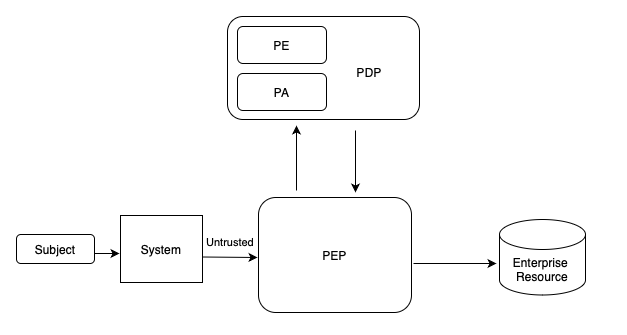
\includegraphics[height=5cm]{./images/architecture}
  \caption{Logical components of ZTA[source: NIST]}
  \label{fig:architecture}
\end{figure}


\subsubsection{Policy Engine}
The Policy Engine (PE) is in charge of deciding whether or not to allow access to a resource for a particular resource.
To give, deny, or revoke access to a resource, the PE employs enterprise policy together with input from external sources 
as input to a trust algorithm. The component of the policy administrator is matched with the PE. 
The decision is made by the policy engine, which also documents its approval or rejection. 
The policy administrator then puts the decision into action.

\subsubsection{Policy Administrator}
The Policy Administrator is the component handling initiation and/or termination of the communication line between a resource and a subject. 
Any session-specific authentication, credential, or token 
that a client uses to get access to an enterprise resource would be generated by it. It is directly related to the PE and 
depends on its final determination of whether to approve or reject a session. The PA sets up the Policy Enforcement Point to permit the session 
to begin if the request has been authenticated and the session is allowed. The PA notifies the PEP to terminate the connection 
in the event that the session is rejected or an earlier approval is overturned.

\subsubsection {Policy Enforcement Point}
The PEP is in charge of permitting and overseeing connections between a subject and an enterprise 
resource. The PEP interacts with the PA in order to transmit requests and/or 
obtain updates on PA policies. Although there is just one logical component in ZTA, it can be divided into two parts: the 
resource side (such as the gateway component in front of the resource that regulates access) and the client 
(such as an agent on a laptop) or a single portal component that serves as a gatekeeper for communication channels. 
The trust zone containing the enterprise resource is located beyond the PEP, as seen in figure 2.1.

[cite NIST here]

\section{Kubernetes}

\subsection{Components}

A Kubernetes cluster is separated into a control plane and a data plane. The control plane
groups the components responsible for the underlying system of Kubernetes itself. The data
plane hosts the actual user containers. Machines that run control-plane services are referred to as master-nodes, 
whereas machines that host user applications are referred to as worker-nodes. There are four core control-plane components
that work together to manage the cluster and ensure that applications run smoothly. These components run as containers
themselves inside the reserved ’kube-system’ namespace. 
\newline
\begin{figure}[htbp]
  \centering
      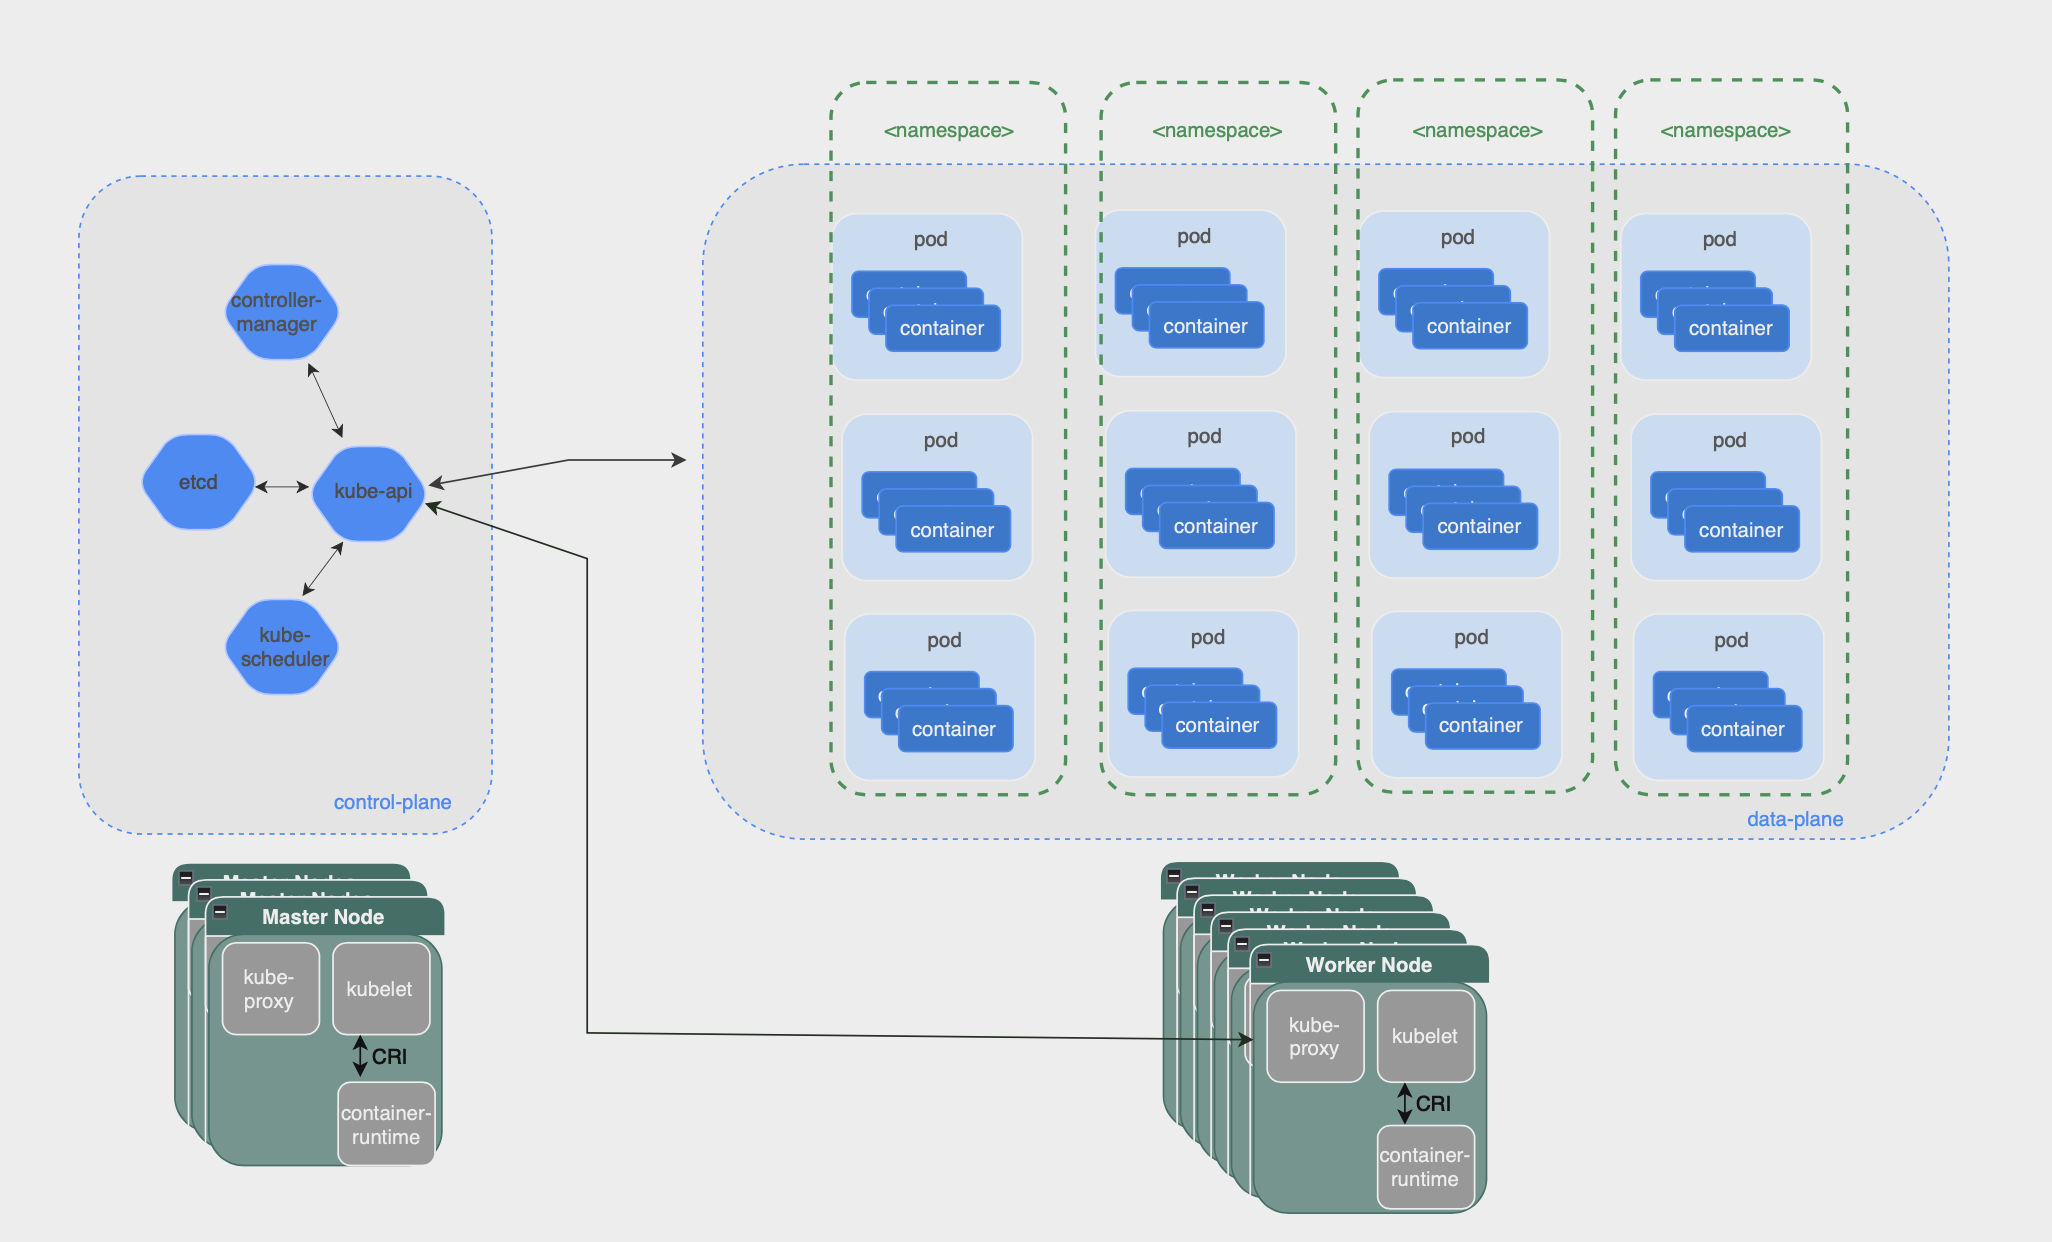
\includegraphics[height=8cm]{./images/kubernetes}
  \caption{Kubernetes Architecture [source: author]}
  \label{fig:architecture}
\end{figure}
\newline
The API server in Kubernetes acts as the gateway, offering a REST API 
through which users and applications can communicate with the cluster, enabling resource management, access control, and 
querying of cluster state and configurations. The Kubelet, an agent process on each node, ensures that pods are running healthy
and up-to-date with the desired state. This is achieved by communicating with the API server.
Etcd, a distributed key-value store, maintains the cluster's consistent state across multiple nodes, utilized by control plane
components for storing cluster information such as resource configurations and pod statuses.
The kube-scheduler allocates pods to nodes based on resource availability and requirements, aiming to optimize successful pod 
execution while enhancing cluster resilience by distributing pods across multiple nodes.
The controller manager, operating on each node, oversees the cluster's state, responds to events like pod creation or deletion, and takes 
corrective measures to maintain cluster health, such as restarting unhealthy pods or scaling to meet demand. [cite k8s docs]

\subsection{Core Cluster Objects}

\subsubsection{Namespaces}
Within a single cluster, resource groups are arranged and separated using namespaces, which are virtual partitions in Kubernetes. 
Namespaces allow the cluster to be logically divided into smaller, more manageable chunks. 
Namespaces are defined by Kubernetes objects such as "Deployment", "Service", and "ConfigMap" to describe an application's state. 
Globally existing and not namespaced objects are those that define the cluster as a whole or that apply to all applications across all namespaces. 
Namespace isolation preserves the integrity of every deployment by averting unintentional interactions or interference between applications. 
Custom authorization rules and access control techniques can be enforced by assigning distinct security policies to namespaces. 
This aids in resource protection and limits unauthorised access between specific namespaces inside the cluster. [cite k8s docs]


\subsubsection{Pods, Replicasets, Deployments, Statefulsets}

In Kubernetes, pods are fundamental building blocks for deploying and managing container-
ized applications. A pod is a unit of one or more containers, which belong together and share
resources such as network namespaces and filesystems. This tight coupling allows pods to be
treated as a single unit for scheduling, management, and resource allocation. Pods expose
the ports exposed by its containers, allowing external traffic to reach its intended recipient.
Pods are rarely instantiated by themselves. Deployments, Replicasets, and Statefulsets are higher 
deployment configurations that specify pod settings. [cite k8s docs]

\subsubsection{ServiceAccount and RBAC}

Pods can use a ServiceAccount as a security identity to access Kubernetes services and resources. 
It controls pod access, permissions, and interactions with the cluster and serves as an authentication method for pods. 
ServiceAccounts have the ability to mount Secrets into Pods, giving them access to private information such certificates, API keys, and passwords.
\newline
RBAC is an authorization system that regulates which individuals or groups can access resources and carry out particular tasks inside the cluster. 
It offers a detailed method for controlling access rights and enforcing security regulations throughout the Kubernetes environment.
Role objects define a set of permissions that can be granted to users or groups. They specify which resources can be accessed, what actions can be performed 
on those resources, and the scope of the permissions (namespace-wide or cluster-wide). ClusterRole objects are similar to Roles, however, they have a broader scope, 
applying to all namespaces within the cluster. They are typically used to define permissions for system components or users who need access to resources across multiple namespaces.
RoleBindings and ClusterRoleBindings assign the designated permissions to users or groups based on the association between Roles or ClusterRoles. 
They specify how identities and the permissions they possess are mapped out. Such RoleBindings are bound to previously mentioned ServiceAccounts. [cite k8s docs]


\subsection{Kubernetes Networking}

A key component of Kubernetes that guarantees smooth communication between containers, pods, and services inside a Kubernetes cluster is Kubernetes networking. 
Networking is made uniform by the Kubernetes network model.

\subsubsection{Pod Networking}
Each pod in Kubernetes has its own IP address. Containers within a pod can freely communicate with one another via localhost. With these pod IP addresses, pods 
can communicate with any other pod in the cluster without requiring Network Address Translation (NAT). Network policies are used to establish pod isolation; 
pods are treated in the same way as virtual machines (VMs) or hosts with distinct IP addresses. Since they operate in the same network namespace, containers inside of 
pods share the IP address of the pod.

\subsubsection{Service and Ingress}
Access to a collection of pods is abstracted by Kubernetes services and is often represented by a virtual IP address within the cluster. Node ports or load balancers 
allow access to these services from outside the cluster. Even when the underlying pods change, a service's virtual IP address and DNS name stay the same. Load balancing and 
flexible access control are thus made possible.

\subsubsection{Container Network Interface (Plugins)}
The Container Network Interface (CNI) API provided by Kubernetes allows for the support of several network solutions. Third-party network implementations are increasingly
utilized, even though Kubernetes' integrated network support, kubenet, provides basic connectivity. Pods can be connected to the network using network plugins, and pod IP addresses 
can be assigned using IP Address Management (IPAM) plugins. Calico and Cilium, for instance, offer flexibility in selecting the optimal networking solutions for certain needs and settings by 
providing both network and IPAM plugins and integrating with other CNI plugins.

[cite tigera, cilium, k8s docs]

\section{Zero Trust versus Traditional Security Model}

in depth here 



\chapter{Creating the Zero Trust Cluster}

\section{Virtual Machines and Network}

The base infrastructure of this thesis project consists of 5 Virtual Machines that are running on a Proxmox infrastructure provided by FH Campus Wien. At the edge of the network sits an OPNsense 
gateway, an open-source firewall based on FreeBSD, which controls external traffic coming into 
this thesis' network. Its external interface on 10.140.0.50 is part of a broader WAN provided by the institution's facilities. This gateway serves as the primary entry and exit point for all traffic 
entering or leaving the internal network, playing a critical role in securing and directing network traffic. The gateway runs a Wireguard agent - the general environment is accessed using SSH through  
a Wireguard VPN tunnel. Since the focus of this thesis lies on the Kubernetes environment, and as OPNsense is not directly 
part of the Kubernetes setup, there shall be no further in-depth description of this OPNsense gateway. 
\newline
\newline
The LAN is segmented into a distinct subnet 192.168.20.0/24. Within this subnet, four VMs have been deployed, each assigned static IP addresses ranging from 192.168.20.1 to 192.168.20.5. 
These VMs serve various roles within the network, hosting different services and agents required for the Kubernetes environment and its Zero Trust character. A static IP address assignment was chosen to ensure consistent network addressing
and to facilitate easier management and configuration of these VMs. The Ubuntu installation wizard was used to complete base configurations such as username, password, hostname, and IP addresses. 
Each of these VMs runs Ubuntu 22.04 LTS, a popular Linux distribution known for its stability, security features, and extensive software repositories. 
This choice of operating system emphasizes a preference for a robust, community-supported platform capable of handling the demands of modern networked applications. 
With 8GB of RAM and 4 CPU cores allocated to each VM, they are well-equipped to run Kubernetes.
\newline
\newline
To give a general overview of the setup, an authentication proxy is deployed on a standalone VM on 192.168.20.2, apart from the Kubernetes cluster itself. The cluster is deployed on the remaining three 
VMs. 192.168.20.3, the master node, is running the control-plane (the "brain" of the cluster), consisting of kube-apiserver, etcd, kube-controller-manager and kube-scheduler. 192.168.20.4 and 192.168.20.5 are dedicated worker 
nodes of the cluster running the data-plane (the "body" of the cluster), hosting deployed containers. Each node runs the Kubelet and the kube-proxy. The cluster is organized in multiple namespaces. The components
and software solutions which ensure a Zero Trust approach are deployed in their respective, dedicated namespaces, such as istio-system, keycloak, and teleport-agent. To mimick actual business software hosted on Kubernetes
and for the sake of demonstration, namespace "neptune" and namespace "jupiter" are created. Each of them run simple deployments such as a Nginx webserver. This setup, as shown in figure 3.1, will be explained in depth in the following sections. 

\begin{figure}[htbp]
  \centering
      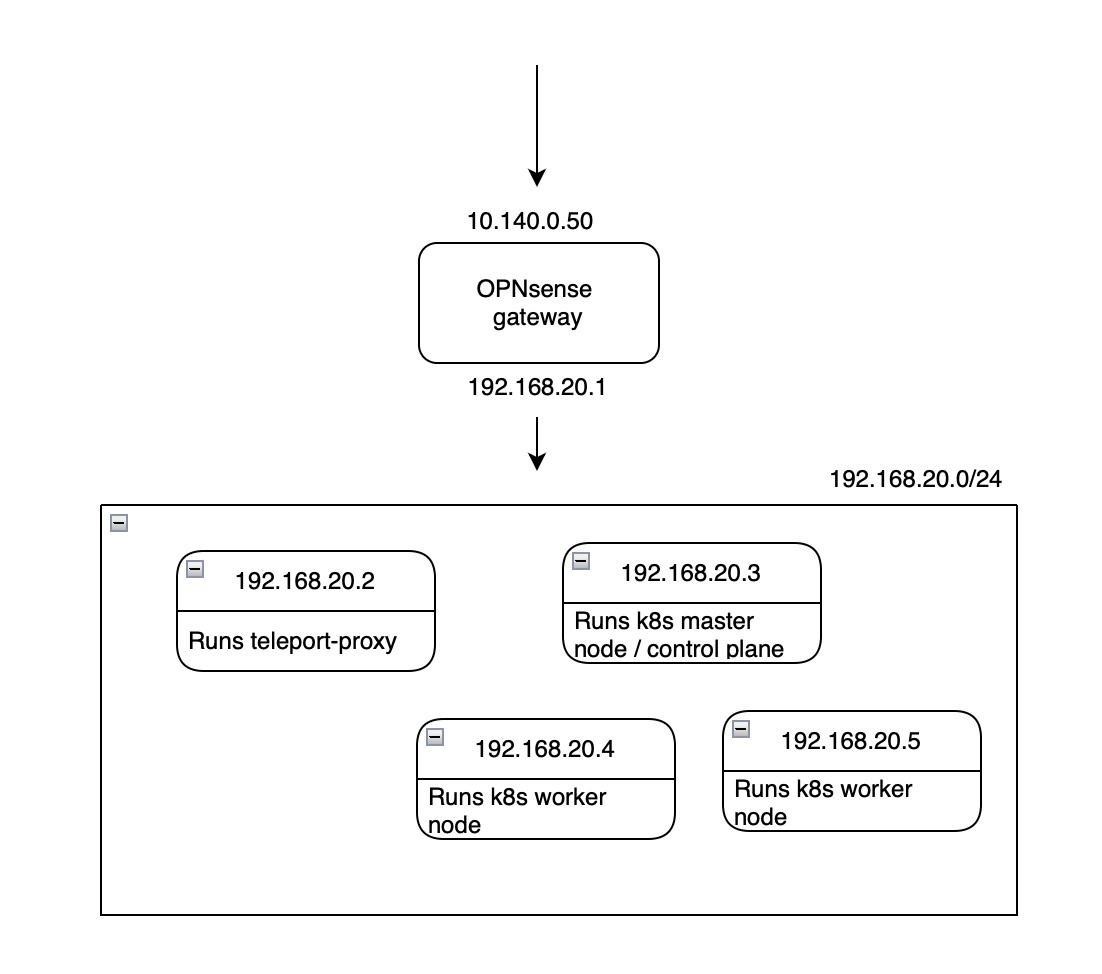
\includegraphics[height=8cm]{./images/setup}
  \caption{General Setup [source: author]}
  \label{fig:generalsetup}
\end{figure}



\section{Bootstrapping the cluster}

Before installing Kubernetes binaries on the nodes, certain settings and kernel parameters need to be configured on the Linux machines that make up the Kubernetes nodes. 
The bash script as seen in figure 3.2 is executed on all three nodes.
\newline
\begin{figure}[htbp]
  \centering
      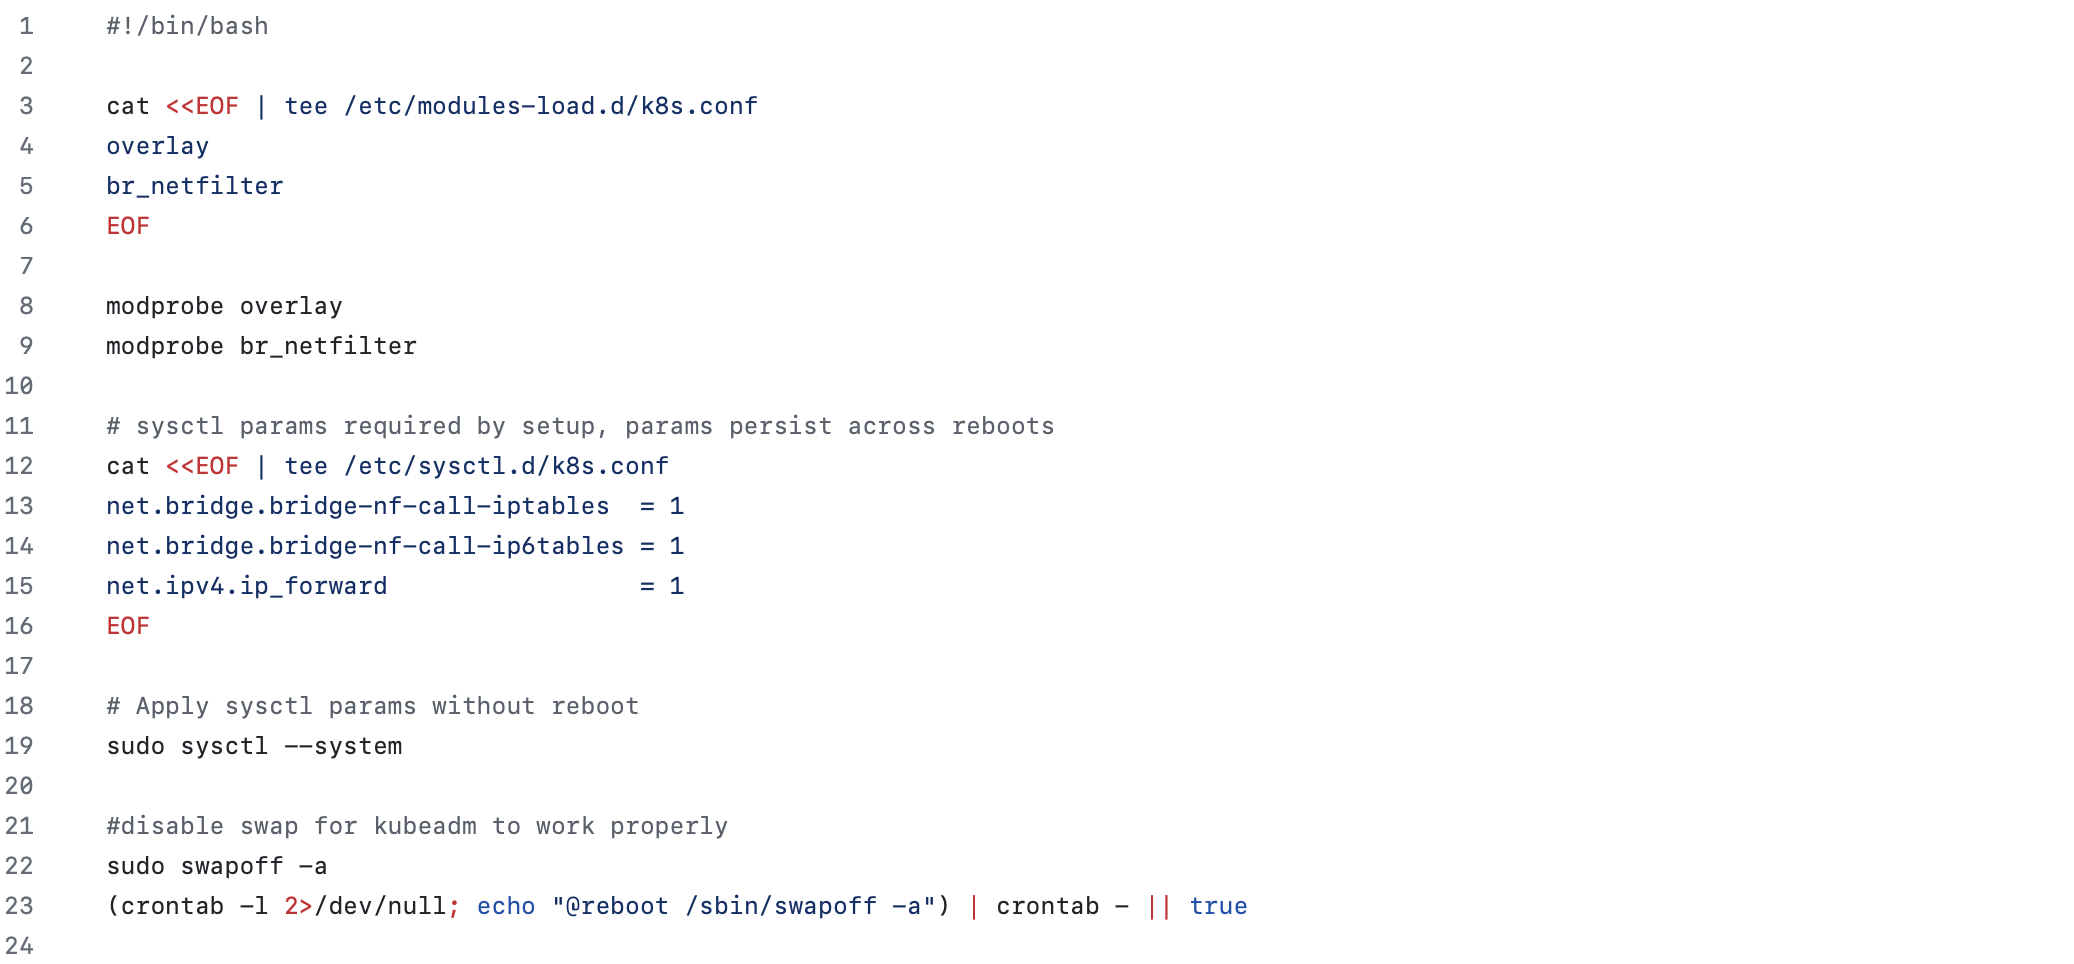
\includegraphics[height=7.8cm]{./images/baseconfig}
  \caption{Base k8s-node configuration [source: author]}
  \label{fig:baseconfig}
\end{figure}
\newline
This script places a k8s.conf file under the /etc/modules-load.d/ directory, specifying overlay and bridge netfilter. This ensures that the kernel modules overlay and bridge netfilter are always loaded at startup of the VM, 
which are required for Kubernetes networking and storage requirement.

\subsubsection{Overlay}
The overlay module is essential for Kubernetes since it activates the overlay storage driver used by container runtimes such as Docker to manage container filesystems efficiently. 
This driver allows containers to share and layer filesystems, optimizing storage use and enhancing performance. By enabling the overlay module, Kubernetes ensures that container runtimes 
can efficiently create, manage, and run containers, which is crucial for the effective functioning of the cluster.

\subsubsection{Bridge Netfilter}
The bridge netfilter module is significant as it allows the Linux bridge to interface with the iptables firewall, enabling packet filtering and NAT. 
This capability is needed for Kubernetes to manage and route network traffic between pods, services, and external networks efficiently. net.bridge.bridge-nf-call-iptables and net.bridge.bridge-nf-call-ip6tables
settings ensure that bridged traffic goes through the iptables chains. net.ipv4.ip-forward enables IP forwarding, allowing the Linux kernel to forward packets between (virtual) network interfaces.
\newline
\newline
With the modprobe command, these modules are loaded into the kernel, making their functions available for use.
Without these settings, Kubernetes components may experience problems with container filesystem management, network packet processing, and general traffic routing.

\subsubsection{Swap}
Disabling swap on Linux during Kubernetes setup, as done in lines 22-23 of Figure 3.2, is necessary because Kubernetes depends on efficient memory management for container orchestration. 
When swap is active, the kernel might swap container memory to disk. 
This results in unpredictable performance and potential container instability. By turning off swap, Kubernetes ensures that container memory stays in physical RAM. 
This allows Kubernetes to manage containers effectively without interference from swapping mechanisms.

\subsubsection{Installation}
After the aforementioned settings, one can proceed with installing the container runtime, kubeadm, kubelet, and kubectl on all nodes. kubeadm is then used to initialize the cluster. kubectl is used to interact with the 
control plane of the cluster. The script as in figure 3.3 downloads GPG keys, installs, and runs CRI-O. Figure 3.4 shows the installation of Kubernetes binaries. Finally, the control plane is initialized on the master node (192.168.20.3), as seen in Figure 3.5, and worker nodes (192.168.20.4 and 192.168.20.5) are joined to the cluster, as seen in figure 3.7.

\begin{figure}[htbp]
  \centering
      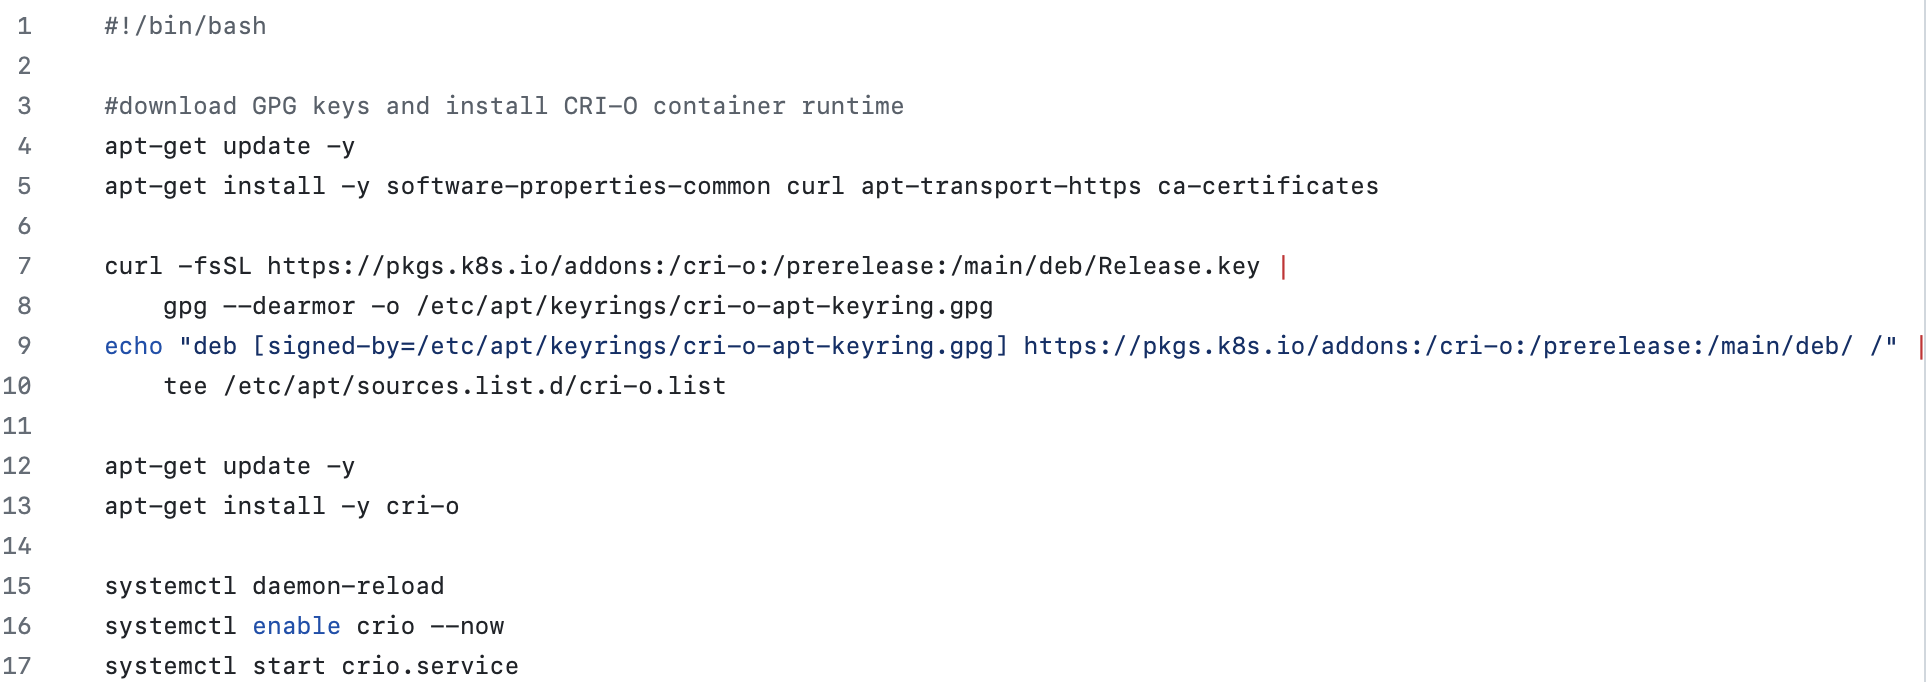
\includegraphics[width=13cm]{./images/crio}
  \caption{Container runtime installation [source: author]}
  \label{fig:crio}
\end{figure}

\begin{figure}[htbp]
  \centering
      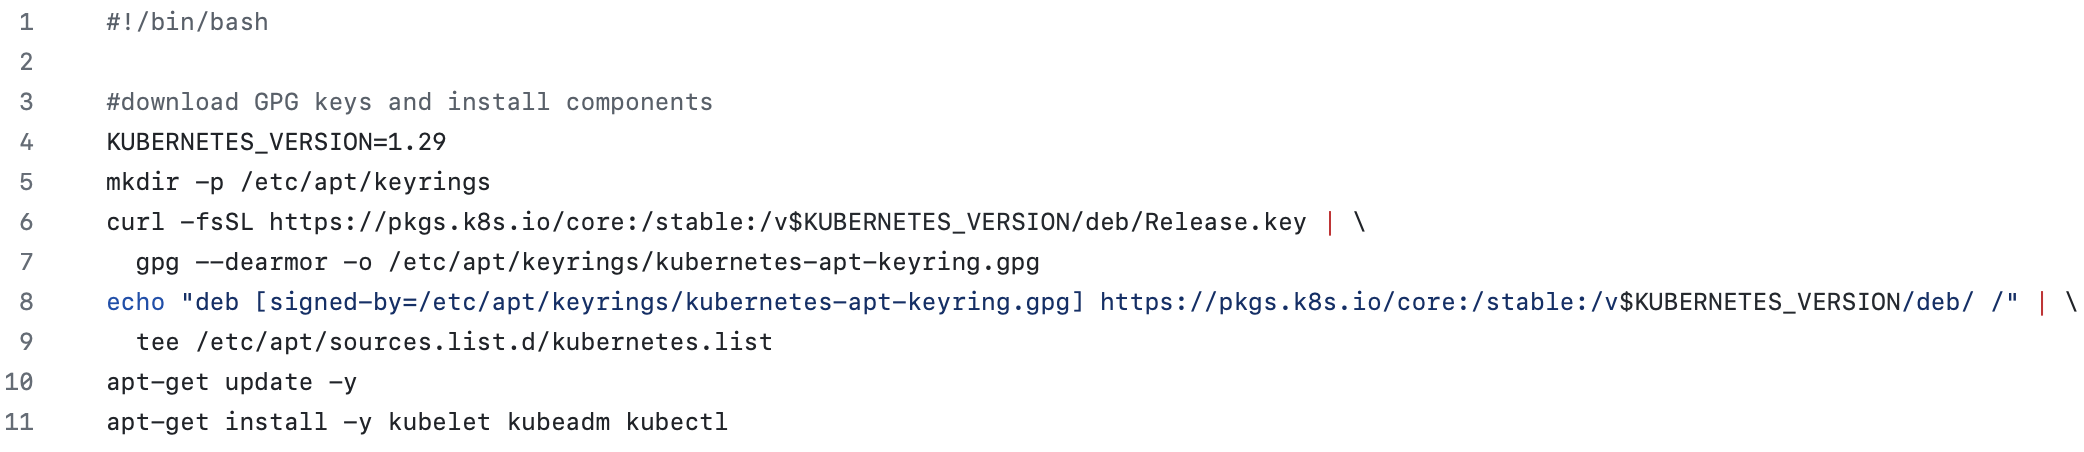
\includegraphics[width=13cm]{./images/k8sbinaries}
  \caption{Kubernetes components installation [source: author]}
  \label{fig:binaries}
\end{figure}

\begin{figure}[htbp]
  \centering
      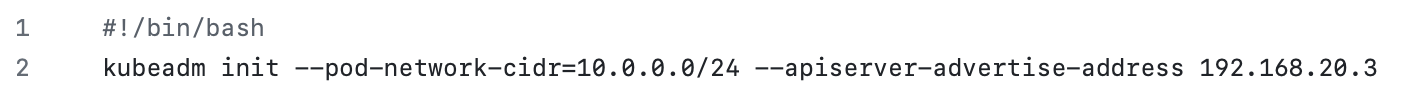
\includegraphics[width=13cm]{./images/master}
  \caption{Control plane initialization [source: author]}
  \label{fig:master}
\end{figure}

\begin{figure}[htbp]
  \centering
      
\includegraphics[width=13cm]{./images/worker}
  \caption{Join nodes to cluster [source: author]}
  \label{fig:worker}
\end{figure}

\newpage
With securely downloaded and installed dependencies in place, the following sections address fortifying the cluster according to Zero Trust principles. 

\section{Teleport}

\subsection{Why use Teleport?}

Kubernetes clusters are administered and accessed by various different professionals: security engineers, database administrators, software developers, DevOps engineers, general system administrators and others. Commandline clients such as 'kubectl' or 'helm' are used to manage the cluster.
Such access must happen in a secure, granular and audited fashion in order for it to fulfill ZT requirements. The default way of accessing the cluster is done by using static client keys and 
certificates placed under .kube/config of the client machine. However, access to the cluster can also happen by means of a dedicated authentication-proxy solution. cite[k8s]
\newline
\newline
Kubeconfig, Teleport, Okta and Hoop are ways of accessing the cluster which were researched for suitability for the setup of this thesis. Kubeconfig means accessing the cluster through a manually issued kubeconfig file. Teleport, Okta and Hoop were identified as authentication-proxy 
solutions to the cluster, aiming to implement ZT. To identify the most appropriate solution for a ZT approach, the following criteria were established: 
\begin{itemize}
	\item Kubernetes friendly
	\item Is free and open source software (FOSS)
	\item Centralized identity management taking care of rotating secrets
	\item Offers Role Based Access Control (RBAC)
	\item Offers Attribute Based Access Control (ABAC)
	\item Provides MFA
	\item Possibility to audit sessions 
\end{itemize}

Out of the box, Kubernetes offers its standard kubeconfig file, consumed by kubectl and helm, to manage Kubernetes clusters. This is inherently Kubernetes friendly, free and open source. This method offers RBAC as part of Kubernetes' integrated RBAC implementation, 
achieved through Role, ClusterRole, RoleBinding and ClusterRoleBinding resources. This method fundamentally lacks the features needed to come closer to a ZT approach. Kubernetes itself does not offer one centralized way of creating, issuing and rotating these credentials. They
are permanently valid until they are manually invalidated, creating a long-lived, single point of compromise. For this reason, authentication proxies such as Teleport, Okta, and Hoop are more appropriate solutions for cluster access. Okta is a mature identity and access management platform
offering strong security features for ZT. It can act as an access gateway in front of Kubernetes clusters. However, this feature is not free and open source software and cannot be self-hosted. It was therefore not taken into further consideration. Hoop.dev and Teleport remain 
as promising solutions. Apart from paid subscriptions they both offer free, self hosted versions and therefore qualify for the setup. The decision for Teleport comes down to the fact that Teleport natively provides even more granular access control through ABAC, implemented by Teleport predicate 
language. 
The comparison is summarized in Figure 3.7.

\begin{figure}[htbp]
  \centering
      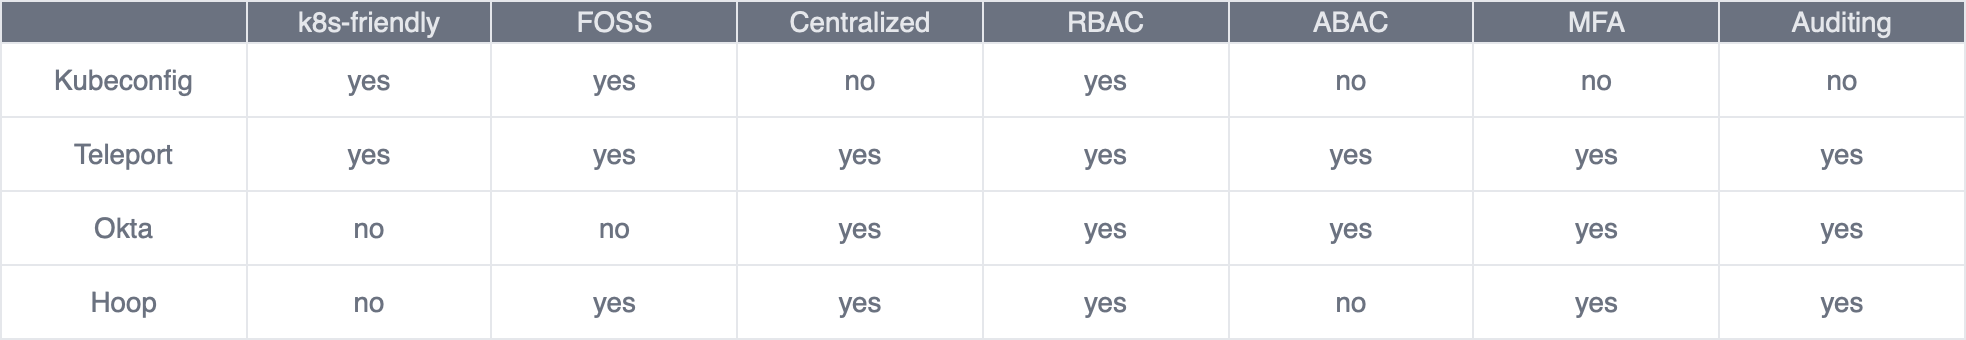
\includegraphics[width=14cm]{./images/tableaccess}
  \caption{Comparison-summary of access solutions to cluster [source: author]}
  \label{fig:tableaccess}
\end{figure}
With Teleport, critical features are implemented, which help shaping the cluster towards Zero Trust. This includes Identity-Driven Authentication, elimination of static credentials, RBAC, ABAC and MFA.

\subsubsection{Identity-Driven Authentication and Authorization}
Teleport acts as a gateway for accessing corporate resources, both on-premises and in the cloud, by leveraging identity-based authentication and authorization. This method eliminates the need for traditional VPNs and password management tools, 
focusing instead on verifying the identity of users rather than their network location or credentials. This approach is central to the Zero Trust philosophy, which grants access based on the identity and purpose of the user, not their physical 
location or network status, as aforementioned in section 2.1. cite[teleport]

\subsubsection{Elimination of Static Credentials}
Teleport issues short-lived identity certificates instead of static credentials. This practice minimizes the risk associated with credential theft, as these certificates automatically expire after a 
certain period, contrasting sharply with the long-term validity of static credentials. This strategy is consistent with the Zero Trust ethos of minimizing vulnerabilities by avoiding the use of persistent secrets. cite[teleport]

\subsubsection{Role and Attribute Based Access Control and Auditing}
Teleport implements role-based access control, allowing access to resources within the corporate infrastructure based on the roles and attributes assigned to individual users' identities. Additionally, it can record all sessions and actions. 
This offers tge ability to monitor and trace access to the infrastructure securely. Such level of control and oversight is crucial for implementing ZT principles, which advocate for continuous verification of access rights and 
thorough monitoring for potential security threats, as mentioned in NIST800-207, and as summarized in chapter two. cite[teleport]

\subsubsection{Public-Facing Proxy and Just-In-Time Access}
Teleport runs a public-facing proxy service that facilitates secure access to resources without the necessity of a VPN. This feature enables just-in-time access, where users are granted temporary privileges to access specific resources or roles as required.
This method strenghtens security by ensuring that users and devices are only granted access based on their immediate needs, reducing the likelihood of unauthorized access or lateral movement within the network. cite[teleport]

\subsubsection{Multi-Factor Authentication}

Multi-Factor Authentication (MFA) is a security measure that requires users to provide two or more verification factors to access a resource such as an application or online account. These factors can include something the user knows (like a password), something 
the user has (such as a security token or a smartphone), or something the user is (fingerprint, facial recognition). By requiring multiple types of verification, MFA significantly increases the difficulty for unauthorized individuals to gain access, even if one 
factor is compromised. This method is a crucial part of Identity and Access Management policies, aiming to enhance security against cyber threats by adding layers of authentication beyond just a username and password. cite[aws]


\subsection{Installation and setup}

Teleport runs on a seperate VM on 192.168.20.2, next to the Kubernetes nodes. The script shown in Figure 3.8...
\begin{enumerate}
	\item Fetches teleports public PGP key
	\item Adds Teleport repository to APT package manager
	\item Installs Teleport
	\item Generates certificate and private key for HTTPS GUI access
	\item Configures and runs Teleport
\end{enumerate}

\begin{figure}[htbp]
  \centering
      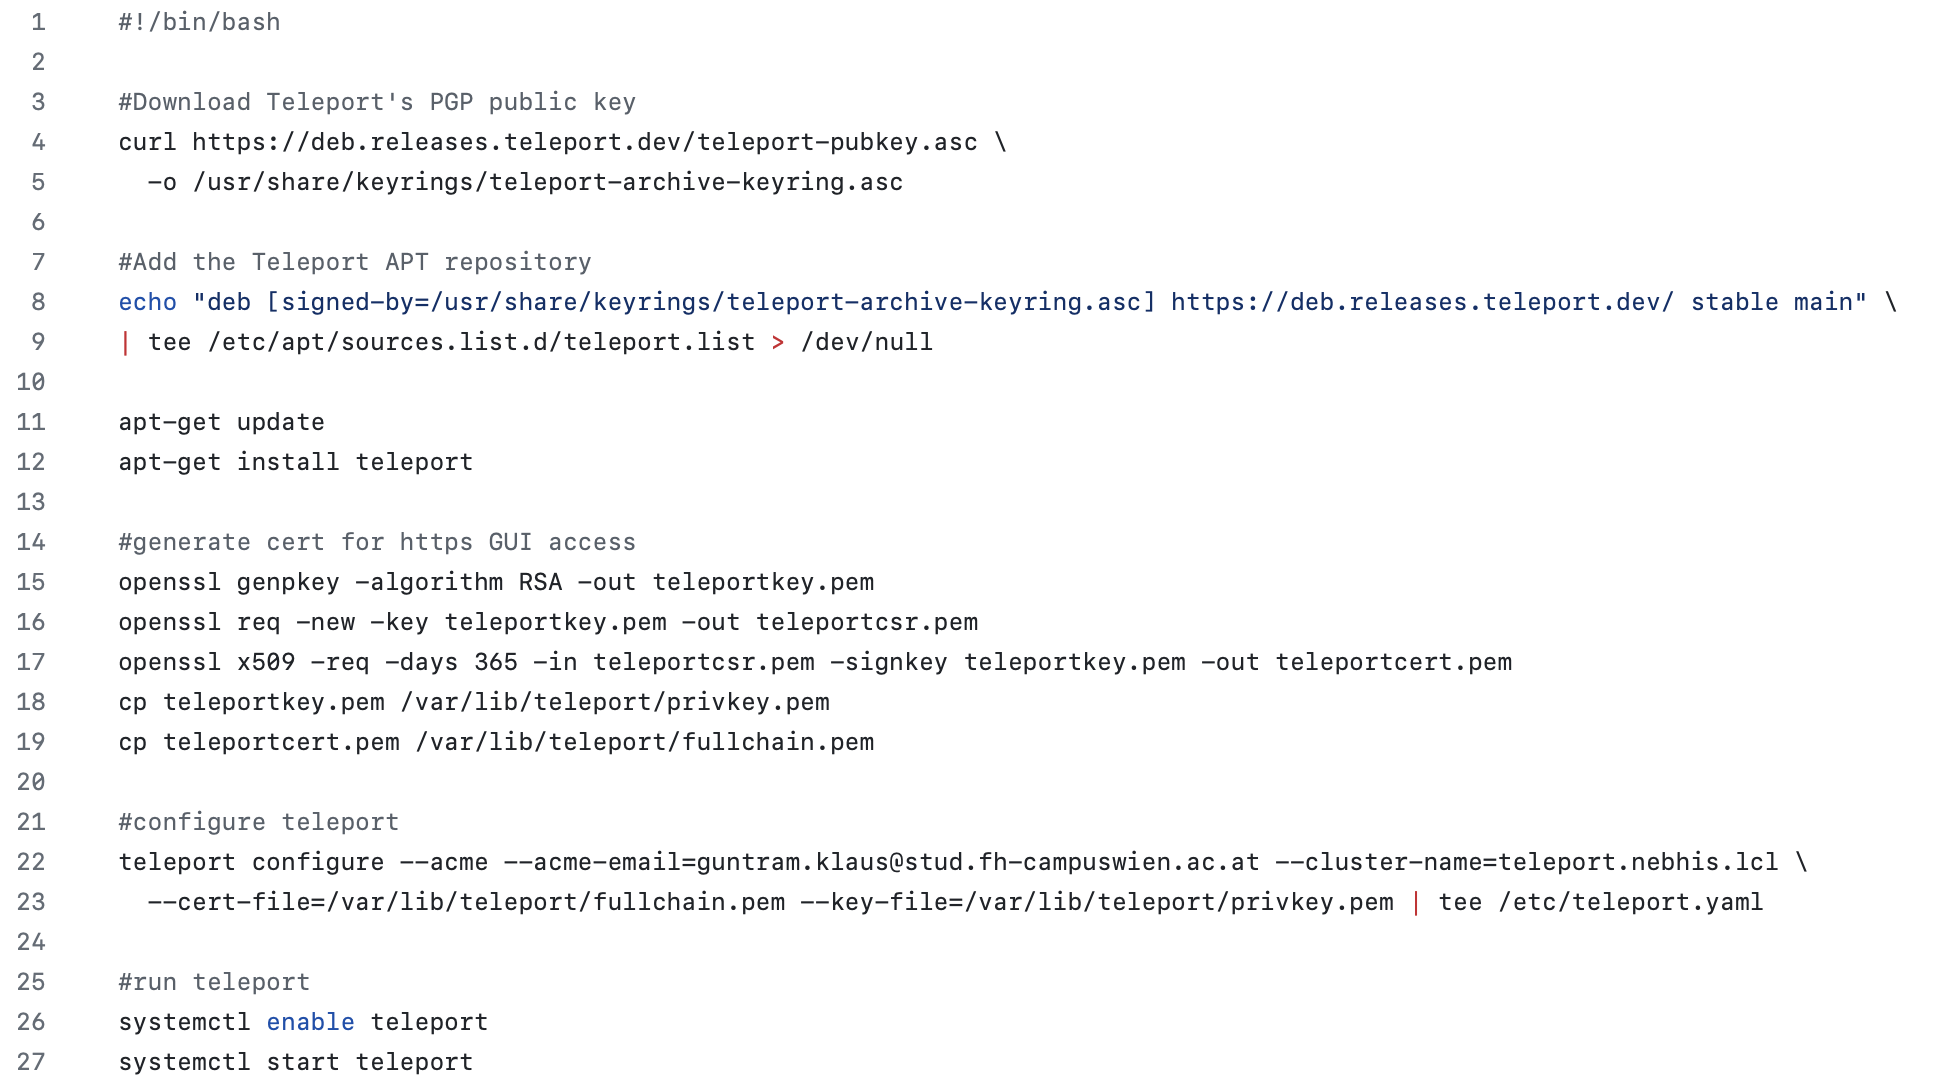
\includegraphics[width=11.5cm]{./images/teleport}
  \caption{Teleport installation [source: author]}
  \label{fig:teleport}
\end{figure}

To enroll the Kubernetes cluster on Teleport, a Helm-based installation was chosen. Helm is a package manager for Kubernetes which simplifies the deployment and management of applications by 
using Helm charts, which are pre-configured templates for Kubernetes resources. It allows for parameterizing Kubernetes YAML definitions. When installing a Helm chart, the parameters of the 
Kubernetes configuration are replaced with concrete values from a dedicated values file. The script in Figure 3.9 takes care of the following things:
\begin{enumerate}
	\item Creates the teleport-agent namespace
	\item Adds the teleport helm chart to the helm repository
	\item Updates and installs the agent using parameters defined in nebhis-cluster-values.yaml, as shown in Figure 3.10.
\end{enumerate}

\begin{figure}[htbp]
  \centering
      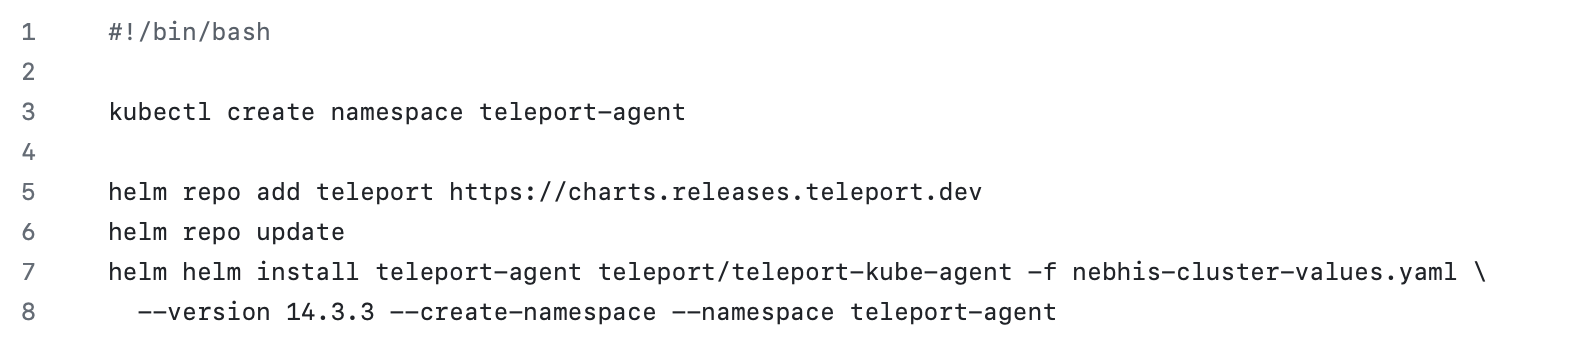
\includegraphics[width=11.5cm]{./images/teleporthelm}
  \caption{Teleport agent installation [source: author]}
  \label{fig:teleportvalues}
\end{figure}

\begin{figure}[htbp]
  \centering
      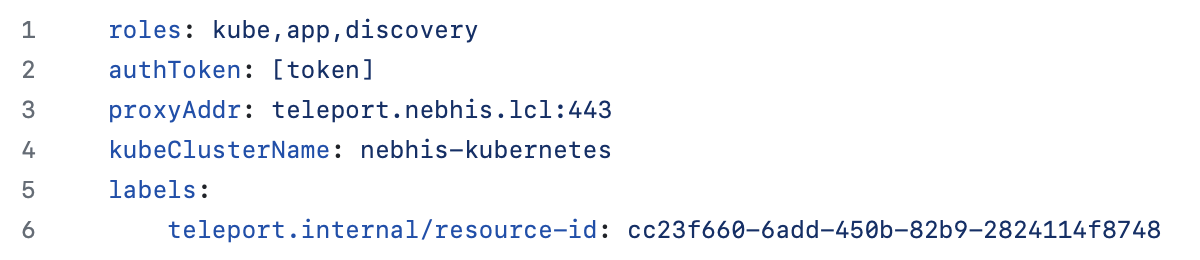
\includegraphics[width=11.5cm]{./images/teleportvalues}
  \caption{Teleport values [source: author]}
  \label{fig:teleportvalues}
\end{figure}

\subsubsection{Authy}

Authy is a mobile application and service that offers two-factor authentication (2FA) for online accounts.
Authy is designed to be compatible with multiple devices, enabling users to synchronize their 2FA tokens across different devices for added convenience and security. 
Teleport requires integration to MFA from the very beginning. When accessing the Teleport UI as well as when using the tsh commandline client, users are prompted for One-Time password tokens (OTP) issued by Authy. 
\newline
\subsubsection{Architecture}
Figure 3.9 provides an overview of the Teleport setup. The key components are the user, the Teleport proxy, 
the Teleport agent, and finally the Kubernetes API server. The user has "tsh" installed on their local machine, 
which is a commandline client used to interact with a given Teleport server. By running "tsh login --proxy=teleport.nebhis.lcl --user=teleport-admin", the user 
"teleport-admin" authenticates to the Teleport cluster "teleport.nebhis.lcl", hosted on 192.168.20.2. This Teleport proxy acts as an intermediary in front of the Kubernetes cluster, enforcing MFA and mTLS. 
Running "tsh kube login nebhis-kubernetes" puts the registered cluster "nebhis-kubernetes" in the current context of the kubectl commandline client by modifying the kubeconfig file under the .kube/config 
directory of the client machine. Subsequently, any Kubernetes API requests executed with kubectl or helm are proxied through the Teleport proxy. 
The Teleport Proxy establishes an encrypted tunnel to the Teleport agent running on a worker node within the "teleport-agent" namespace inside the Kubernetes cluster. 
Finally, the Teleport agent forwards requests to the Kubernetes API Server, which ultimately processes the requests and manages cluster resources. The API server is running on the master node inside the "kube-system" control plane namespace.
This means that the Teleport proxy authenticates the actions "tsh login" and "tsh kube login", and then establishes an encrypted tunnel to 
the teleport-agent, which issues the kubectl command to the API. The respective responsibilities of the proxy and the agent are: 
\newline
\newline
Teleport Proxy:
\begin{itemize}
	\item Authentication and Authorization, check if user is eligible for Kubernetes access
	\item Reverse proxying for Kubernetes API requests
	\item Audit logging and traffic encryption
\end{itemize}

Teleport Agent:
\begin{itemize}
	\item Registering the Kubernetes cluster with the proxy
	\item Manage service accounts and their credentials for Teleport to interact with the Kubernetes API
	\item Synchronize configurations between the Kubernetes cluster and the Teleport Proxy
\end{itemize}



\begin{figure}[htbp]
  \centering
      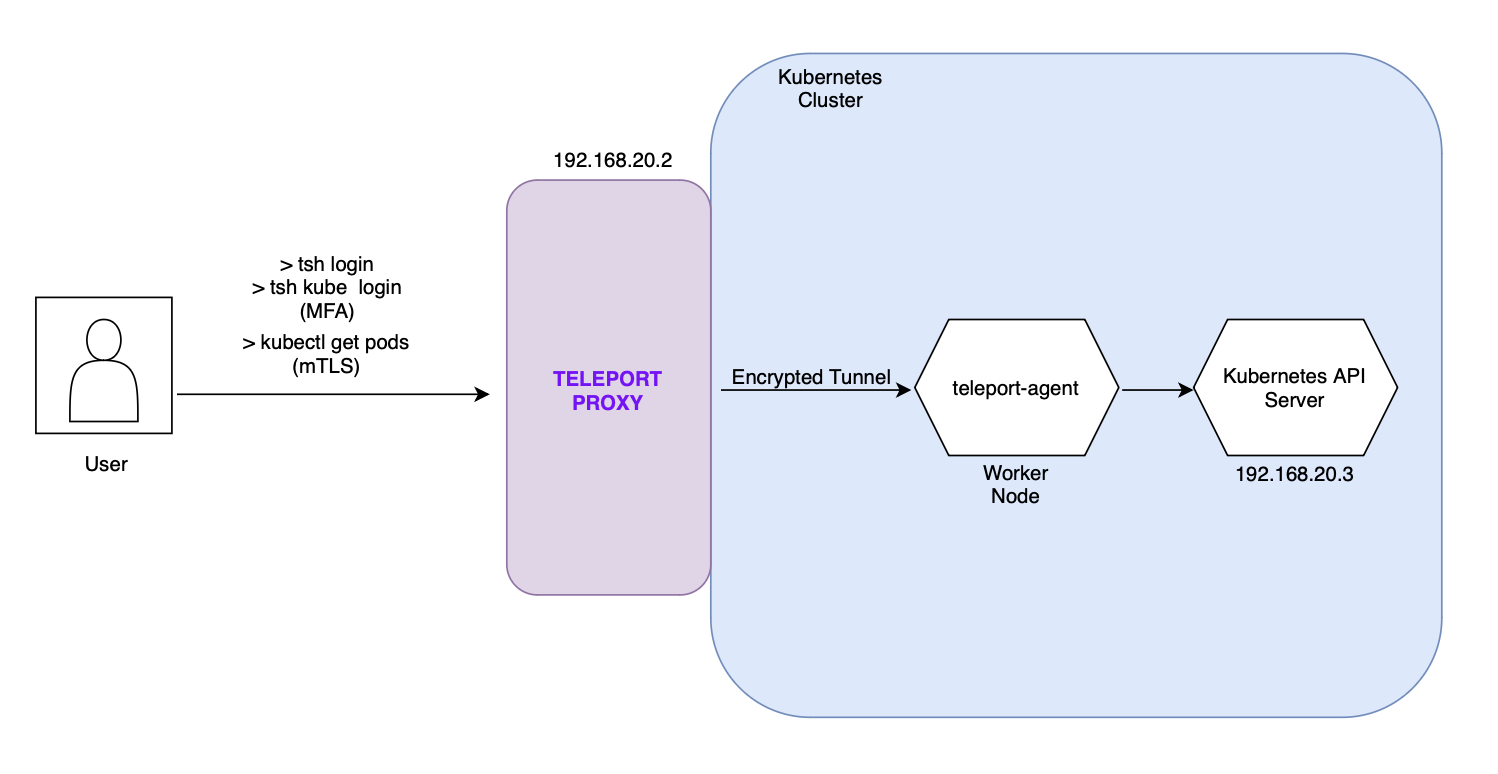
\includegraphics[width=10cm]{./images/teleportarch}
  \caption{Teleport Kubernetes Setup [source: author]}
  \label{fig:teleportarch}
\end{figure}

Thus, access to the cluster covers most of ZT principles as described in NIST800-207. 

\newpage
\section{Istio}

\subsection{Service Meshes}

In a microservices architecture, a service mesh is a special infrastructure layer integrated into an application that manages service-to-service communication. It finds other services, encrypts data, manages the flow of service requests to other services, 
and does load balancing. This is accomplished by injecting a so called proxy sidecar-container into Kubernetes pods. These sidecars intercept any incoming and outgoing traffic of the actual app container. That way, any logic driving matters of network communication
is taken out of the app container and handled on its own plane of infrastructure. These sidecars deployed alongside app containers comprise the data-plane, while the control plane instance usually resides in its own dedicated namespace. The main benefits of 
a sidecar approach are sophisticated routing capabilities, separation of concerns and enhanced security. cite[redhat] cite[istiodocs]
cite[dynatrace]

\begin{figure}[htbp]
  \centering
      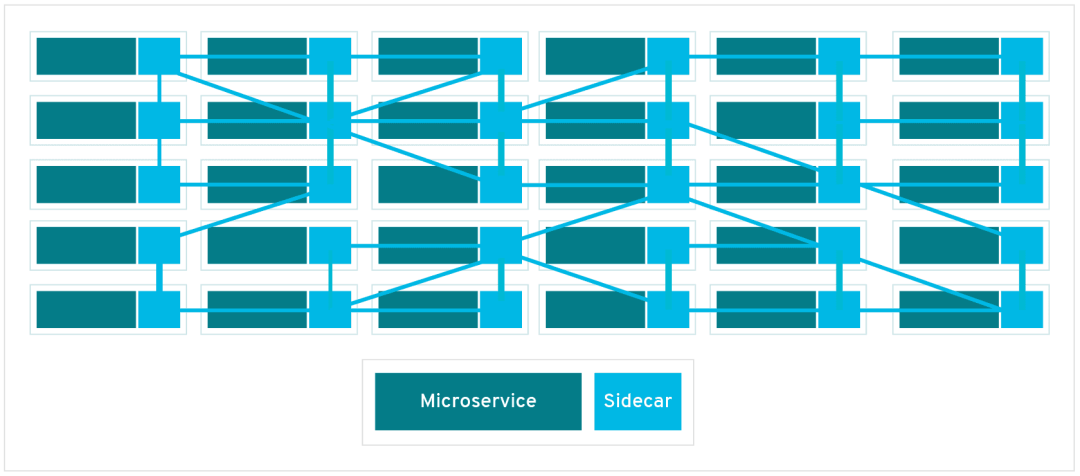
\includegraphics[width=11cm]{./images/mesh}
  \caption{Service Mesh visualization [source: RedHat]}
  \label{fig:servicemesh}
\end{figure}

\subsection{mTLS}

Transport Layer Security (TLS) is a widely used encryption protocol that authenticates servers and encrypts communication between clients and servers, ensuring data privacy and integrity. It operates using public key cryptography, 
which involves a pair of keys: a public key for encryption and a private key for decryption. Mutual TLS (mTLS) extends this concept by requiring both the client and server to authenticate each other using their respective TLS certificates. 
This mutual authentication adds a layer of security, verifying the identities of both parties and enhancing the protection against various cyber attacks. This makes it especially useful in Zero Trust architectures. Since service meshes handle network
communication between pods, they must have the possibility for mTLS to be considered an employable component for a ZT Kubernetes cluster.

\subsection{Why use Istio?}

There are several ways of implementing a service mesh and there are different technologies to realize a service mesh on top of Kubernetes. Linkerd, Consul, Istio, and Cilium Service Mesh are mature, free, and open source software solutions that were taken
into consideration for this thesis. The decision was based on the following criteria. 
\begin{itemize}
	\item Granularity of traffic routing
	\item Option for mTLS
	\item OIDC integration
	\item Audit logging 
	\item Access logging
\end{itemize}

According to the documentation, mTLS and access logging are provided by all solutions. Audit logging is not natively supported by any of the four solutions. Therefore it comes down to the degrees of granularity offered by the service meshes.
To evaluate granularity, the adjectives 'weak', 'limited' and 'strong' are used. The granularity of traffic routing pertains to how detailed cluster traffic can be controlled as it moves from its origin pod to its destination pod. For traffic routing, each service mesh
solution provides its set of resources with which rules are defined. Controlling traffic in Linkerd is achieved through a combination of the resources ServiceProfile, TrafficSplit, Server and ServerAuthorization. Through these definitions, Linkerd allows to regulate
traffic only based on a service's mTLS identity. It does not offer regulating traffic based on definite IP addresses, native Kubernetes service accounts, namespaces, HTTP methods or OIDC credentials. Consul leverages its service-intentions, service-resolvers, 
service-splitters and service-routers resources which allow for blocking traffic based on IP address and HTTP method. However, it does not natively understand underlying namespaces, service accounts and OIDC credentials. Cilium's service mesh is special as it does not
inject sidecars. Rather, it leverages eBPF Linux kernel technology, which allows for running custom modules in kernel space of the node. This eBPF program, the Cilium agent, implements rules specified in CiliumNetworkPolicy resources. Cilium natively supports the concept of 
Kubernetes namespaces and service accounts. It is possible to allow or deny traffic based on namespace, IP address, service account and HTTP method. However, to validate OIDC credentials, Cilium requires additional integration and configuration with other technologies. 
Istio was found to support all these factors. Istio's VirtualService, DestinationRule, AuthorizationPolicy and RequestAuthentication resources enable traffic controlling also based on provided JWT tokens of the OIDC protocol, on top of other factors such as HTTP method and
namespace. Linkerd and Ciliums eBPF mesh triumphs in terms of performance and efficiency, but not in terms of granularity and security. The degree of granularity offered by Istio could not be found in the other mentioned projects. It is therefore attributed with 'strong'
granularity while Consul, Cilium and Linkerd are marked as 'Limited'. As such, Istio is the chosen solution for the setup. 
The findings are summarized in Figure 3.10.

\begin{figure}[htbp]
  \centering
      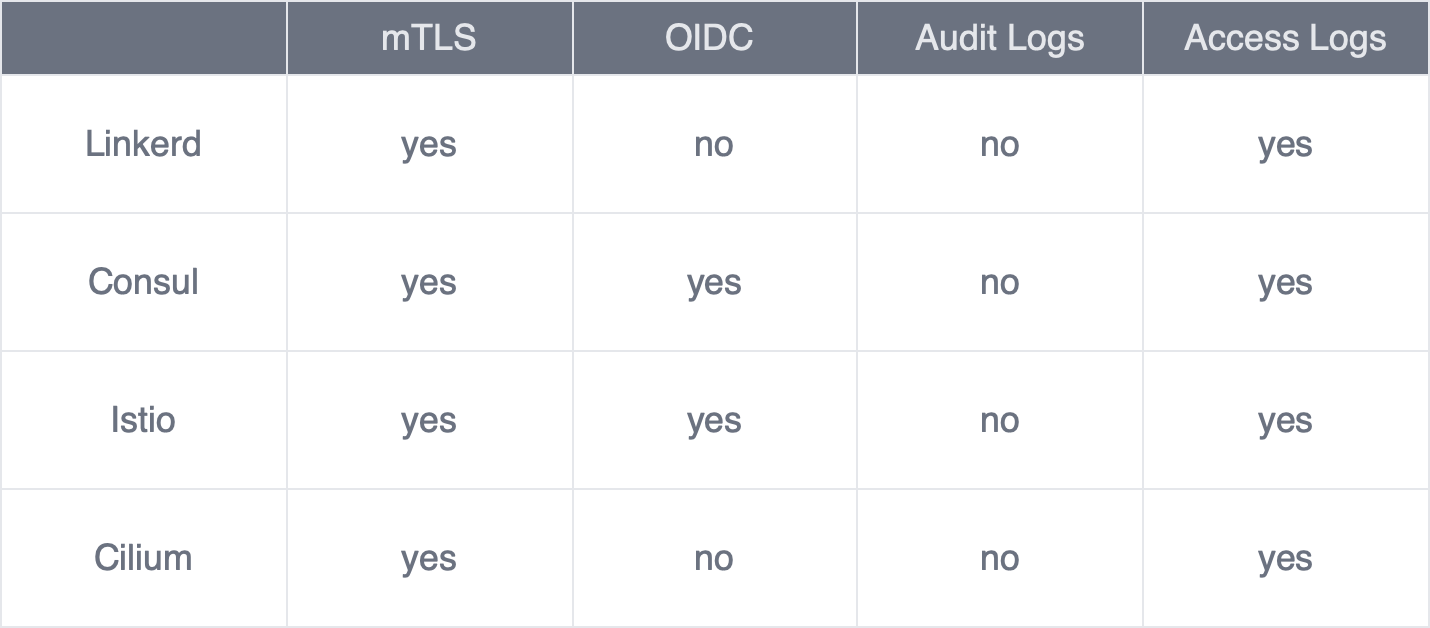
\includegraphics[width=13cm]{./images/tablemesh}
  \caption{Comparison-summary of service-mesh solutions [source: author]}
  \label{fig:tablemesh}
\end{figure}

\newpage
\subsection{Installation and setup}

Like the Teleport agent, Istio was installed using its officially provided Helm chart. First, custom resource definitions (CRD) need to be added to Kubernetes. CRDs allow to extend the Kubernetes API with additional objects beyond the default ones, as
outlined in section 2.2.2 "Core Cluster Objects". Using the script shown in Figure 3.14... 

\begin{enumerate}
	\item Namespace istio-system is created
	\item Istio Helm charts are added to the Helm repository
	\item Istio-base is installed, rolling out CRDs 
	\item Istiod service is installed (control plane)
	\item Istio-ingressgateway is installed in a separate namespace, controlling traffic entering the cluster
\end{enumerate}

\begin{figure}[htbp]
  \centering
      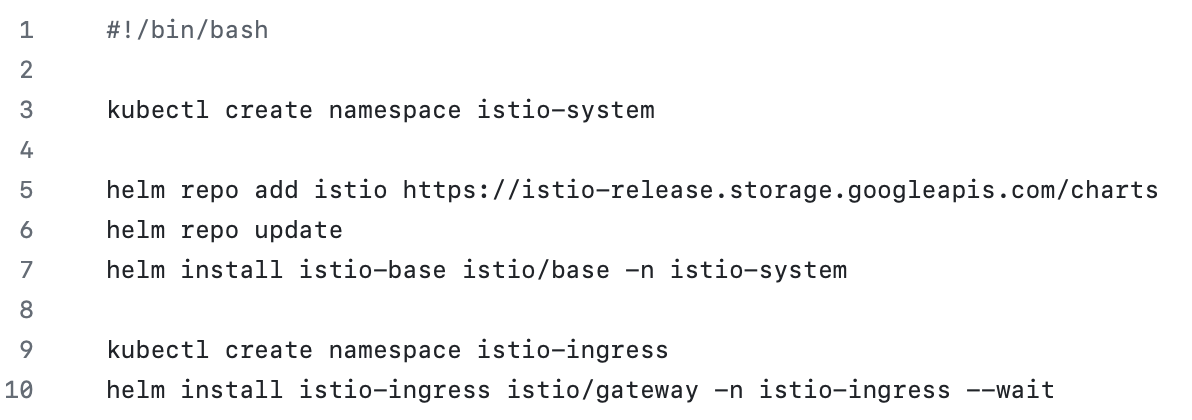
\includegraphics[width=13cm]{./images/istioinstall}
  \caption{Installing Istio components [source: author]}
  \label{fig:istioinstall}
\end{figure}

\subsubsection{Architecture}
Istiod is the central component of the Istio service mesh architecture, responsible for managing the configuration and operation of the service mesh. 
It handles configuration management by distributing configuration information to the Envoy proxies, ensures service discovery by keeping track of all 
services in the cluster, and manages security through the creation, distribution, and rotation of certificates for securing communications within the mesh. 
Additionally, Istiod collects telemetry data from the proxies for monitoring and analysis, and automates the injection of Envoy sidecar proxies into Kubernetes pods, ensuring that all traffic flows through the mesh.
\newline
\newline
The Istio IngressGateway is a critical component of the Istio service mesh that manages incoming traffic from outside the cluster, providing a gateway for external traffic into the mesh. 
It handles traffic management by routing incoming requests to the appropriate services based on configured rules, supports load balancing and enforces authentication and authorization policies.
Istio's architecture including its Ingressgateway, sidecars, and control plane is depicted in Figure 3.15.

\begin{figure}[htbp]
  \centering
      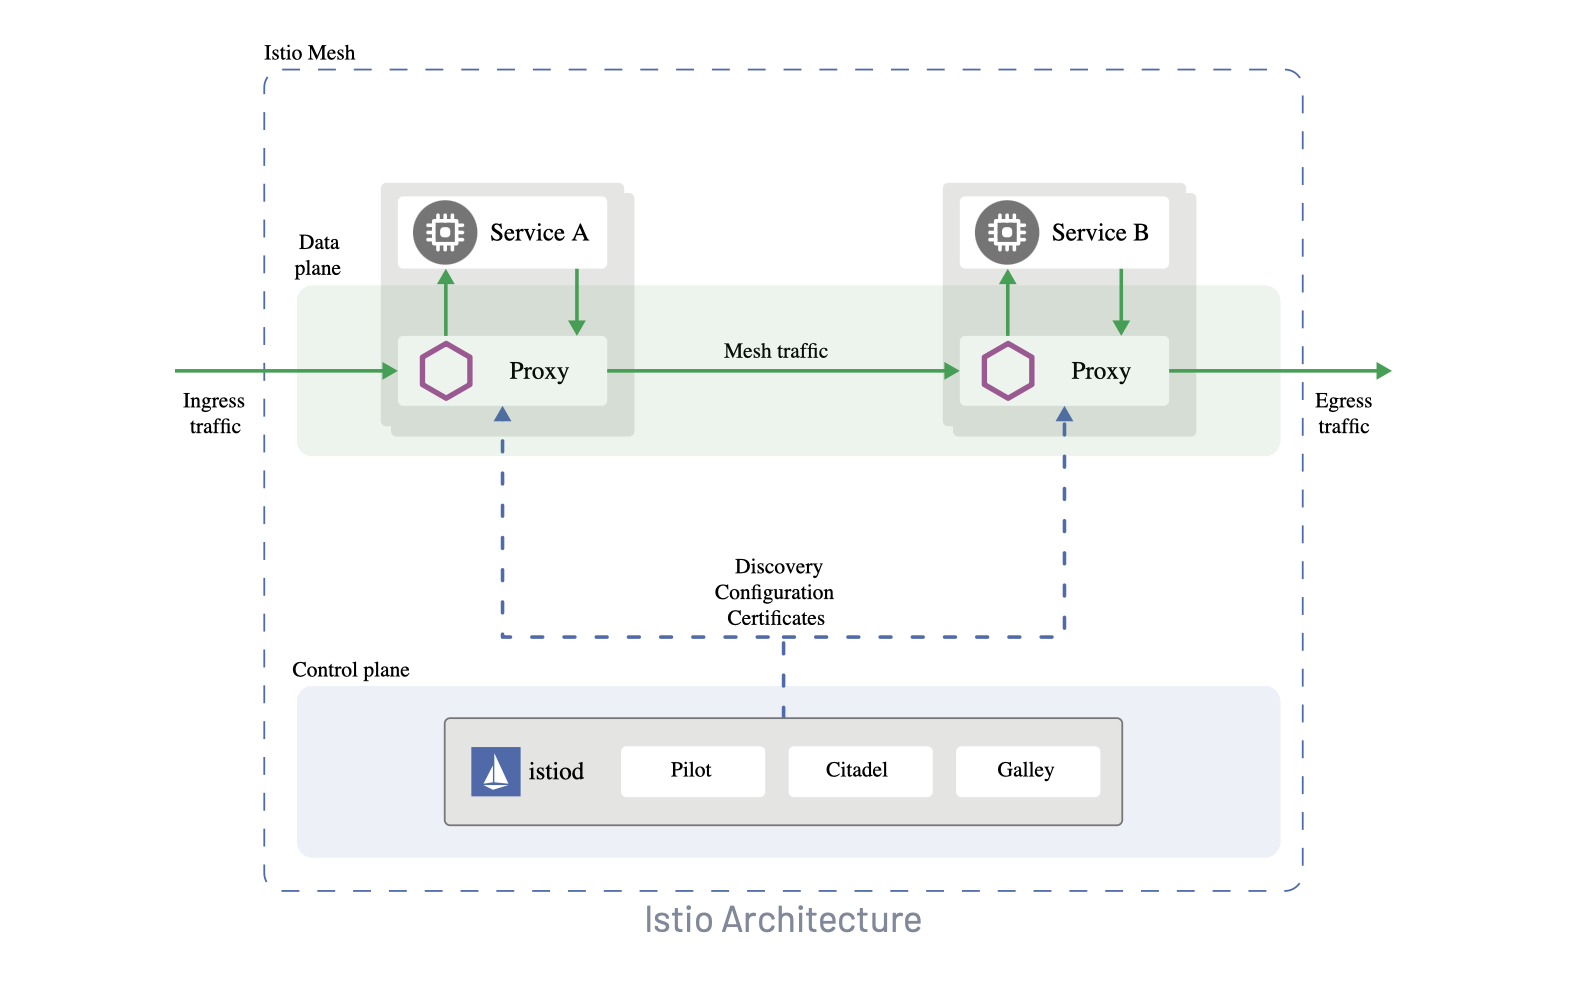
\includegraphics[width=13cm]{./images/istioarchitecture}
  \caption{Istio architecture [source: author]}
  \label{fig:istioarchitecture}
\end{figure}





\section{Keycloak}

\subsection{Identity and Access Management}

IAM refers to all policies, processes and technologies used control access to digital resources. Through IAM systems, it is ensured that only appropriate clients have access to resources under right circumstances. 
For this thesis, IAM is implemented for authorized and granular pod to pod communication. In this context, the term "client" refers to a service issuing a HTTP request to another service hosted in the cluster.
Using a IAM solution, the following things are taken care of. 
\begin{itemize}
	\item Identity Management: Creating client identities and their attributes.
	\item Authentication: Verifying the identity of clients before granting access.
	\item Authorization: Determining what resources an authenticated client or device can access and what actions they can perform.
	\item Access Control: Policies and rules enforcing which clients can access which resources under which conditions.
	\item Auditing: Logging client access and activities to ensure compliance and security.
\end{itemize}

The main drivers of IAM are the concepts of role-based and attribute-based access controls and the protocols Open ID Connect as well as OAuth2. 

\subsection{RBAC and ABAC}
Role-Based Access Control (RBAC) is a commonly implemented access control model that allocates permissions to users based on their organizational roles. In RBAC, roles are defined by job functions, and users receive access to resources and actions that correspond to 
their roles. This model simplifies administration by enabling system administrators to manage permissions via roles instead of individual user basis. For instance, a software developer might have a role that permits access to certain repositories, whereas a
database administrator might have a role that allows access to certain databases and system maintenance tools. The main benefit of RBAC is its ease of implementation and scalability in organizations with clear hierarchical structures.
\newline
Attribute-Based Access Control (ABAC) is a more adaptable and flexible access control model that grants access based on a combination of attributes about the user, the resource, and the environment. These attributes can include user details (such as department, job title, or clearance level), 
resource characteristics (such as data sensitivity or classification), and contextual factors (such as time of day or location). ABAC policies leverage these attributes to create intricate, fine-grained rules for access control. For instance, an ABAC policy might permit a system engineer to access 
certain servers only during business hours and exclusively from within the corporate network. This degree of granularity makes ABAC effective in environments where access requirements are complex and highly variable.
\newline
ABAC is more suitable for ZT because it provides the flexibility and granularity needed to implement dynamic and context-aware access controls essential for ZT. Unlike RBAC, which is relatively static and role-centric, ABAC can evaluate multiple attributes in real-time to 
determine access permissions, ensuring that only authenticated and authorized users can access resources under specific conditions. This aligns with ZT's core tenet of minimizing trust and continuously verifying every access request based on a comprehensive set of criteria, 
thereby enhancing security and reducing the risk of unauthorized access.

\subsection{OIDC and OAuth2}

OpenID Connect (OIDC) and OAuth 2.0 are complementary protocols that together provide a framework for authentication and authorization on the web. OAuth 2.0 is the de facto standard authorization framework that allows third-party applications to 
obtain limited access to a web service, either on behalf of a resource owner or by allowing the third-party application to access its own resources. It works by issuing tokens that represent the user's delegated permissions, enabling secure access
without sharing passwords. OpenID Connect, built on top of OAuth 2.0, extends this protocol by adding an identity layer, allowing applications to verify the identity of the end-user based on the authentication performed by an authorization server. 
OIDC standardizes the way identity information is exchanged using RESTful APIs, providing user profile information through an ID token. This integration of OIDC and OAuth 2.0 ensures that while OAuth 2.0 handles authorization and secure resource access, 
OIDC handles user authentication and identity management.

\subsubsection{Pod to pod OIDC flow}
In the context of this thesis, a service running inside the Kubernetes cluster may only access another service if the request contains a valid OIDC token, as done through the following steps. 

\begin{enumerate}
	\item The client service sends a POST request to the authorization server's token endpoint. This request contains the clientID, a client secret, and the grant type.
	\item The authorization server validates the client secret and issues a short-lived access token. 
	\item The client receives the token and adds it to subsequent requests to the resource server. The token is added in the 'Authorization' HTTP header. 
	\item The resource server validates the access token by veryfying its signature, using the public key obtained from the PKI endpoint of the authorization server. If the token is valid, the resource server returns the requested resource. 
\end{enumerate}

However, in this thesis' setup, the validation of the access token is not done by the resource service itself. This step is done by the Istio service mesh. The Istio sidecar-proxy in every appliaction pod abstracts this handling of OIDC tokens. That way,
a request does not even reach the resource server in case of invalid credentials. 

\subsection{Why use Keycloak?}

Authentik, Keycloak, Gluu and Okta are four IAM solutions which were inspected for the following criteria. 
\begin{itemize}
	\item Free and open source software (FOSS) 
	\item OAuth2 support
	\item OIDC support
	\item MFA support
	\item Degree of granularity
	\item Option for auditing
\end{itemize}



Based on the documentations, all four solutions have comprehensive offerings for above mentioned criteria. OAuth2, OIDC, MFA and extensive granularity have become non-negotiable features of proper IAM solutions and are 
achieved in equal measure across Authentik, Okta, Keycloak and Gluu. Out of these, there is no product which unambiguously surpasses the other when it comes to the requirements of this setup specifically. Nonetheless, 
Keycloak was chosen because of its substantial community support on GitHub issues and StackOverflow, its great Kubernetes compatibility due to officially provided Helm charts and its clear, extensive documentation. 

\begin{figure}[htbp]
  \centering
      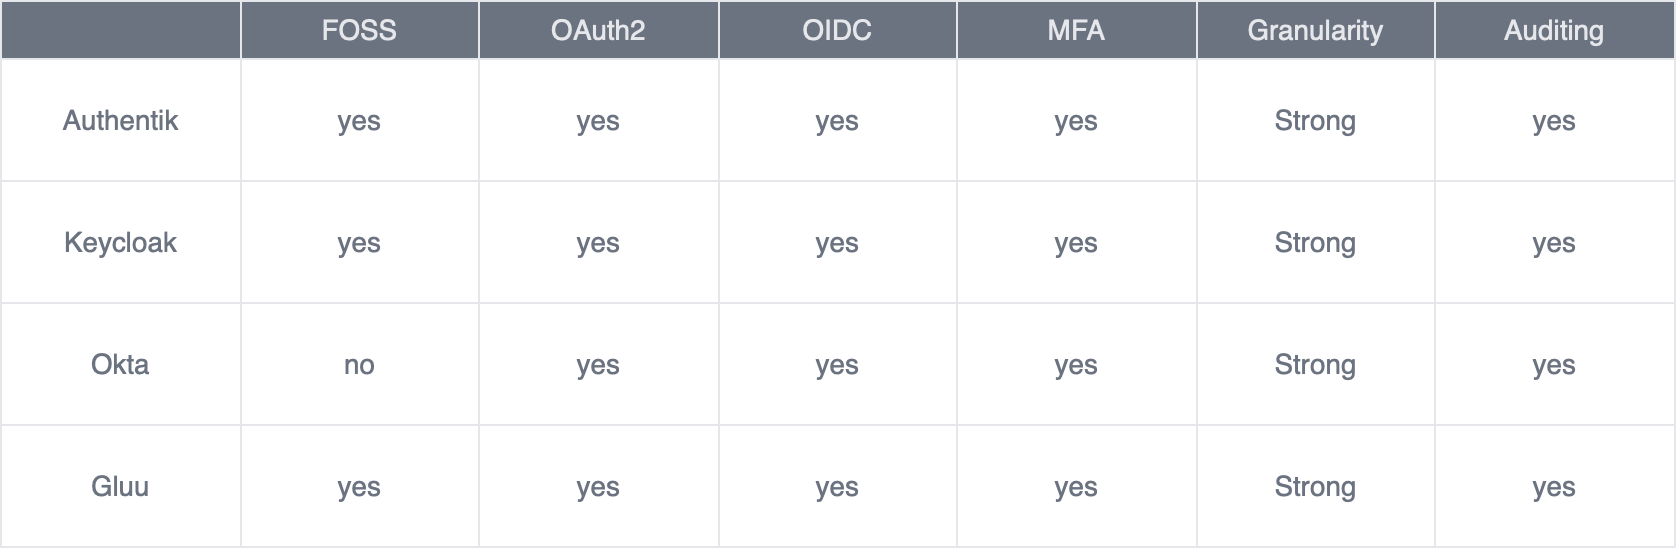
\includegraphics[width=13cm]{./images/tableiam}
  \caption{Comparison-summary of IAM solutions [source: author]}
  \label{fig:tableiam}
\end{figure}

\subsection{Installation and setup}

Keycloak was installed using Kubernetes manifests directly, by issuing "kubectl apply" commands. The Keycloak Docker image provided by Bitnami is used in the deployment object. 
Within the cluster, the Keycloak pod is exposed via a service object named "keycloak-service". Hence, applications can reach Keycloak under the cluster domain "keycloak-service.keycloak.svc.cluster.local".

\begin{figure}[htbp]
  \centering
      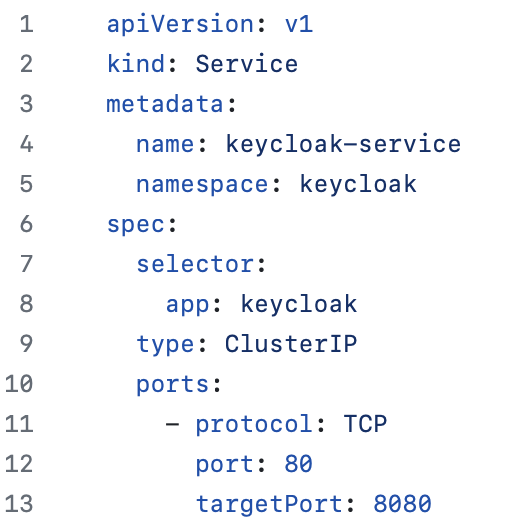
\includegraphics[width=5cm]{./images/keycloakservice}
  \caption{Service object exposing Keycloak [source: author]}
  \label{fig:keycloakservice}
\end{figure}

An application realm called 'nebhis' was created inside the Keycloak UI, which is used for creating Keycloak clients. For this realm, Keycloak provides two central realms for the ZT setup:

\begin{itemize}
	\item keycloak-service.keycloak.svc.cluster.local/realms/nebhis/protocol/openid-connect/token. This endpoint is consumed by applications requesting an OIDC token, to be further used to authenticate to other applications in the cluster.
	\item keycloak-service.keycloak.svc.cluster.local/realms/nebhis/protocol/openid-connect/certs. This endpoint is consumed by the Istio service mesh. The sidecar intercepts incoming traffic to an application pod, extracts the token from the 'Authorization' HTTP header, 
        and validates it using the PKI information obtained under this endpoint. 
\end{itemize}

\subsubsection{Keycloak combined with Istio}

With Istio's service mesh capabilities and Keycloak as an identity provider running in the cluster setup, tightly regulated traffic controls with aforementioned AuthorizationPolicy and RequestAuthentication policies can be achieved.
Together, they act as the logical components "Policy Decision Point" and "Policy Enforcement Point" of a ZT architecture as described in section 2.1.3. 
Istio, as a service mesh, acts as the PEP. The sidecar proxies administered by the control plane intercept incoming and outgoing traffic of a Kubernetes pod. The intercepted traffic is handled according to
configurations made in Istio's AuthorizationPolicy and RequestAuthentication resource. Keycloak serves as the PDP.  It issues JWT tokens after authenticating users and can embed user claims, roles, and other identity information within these tokens.
The AuthorizationPolicy shown in figure 3.18 declares that the "jupiter" service within the "jupiter" namespace may only be accessed, if the request contains a JWT tokens issued by the keycloak service hosted on "keycloak-service.keycloak.svc.cluster.local", for the realm "nebhis".
Istio validates the JWT according to specifications of RequestAuthentication shown in figure 3.19. 

\begin{figure}[htbp]
  \centering
      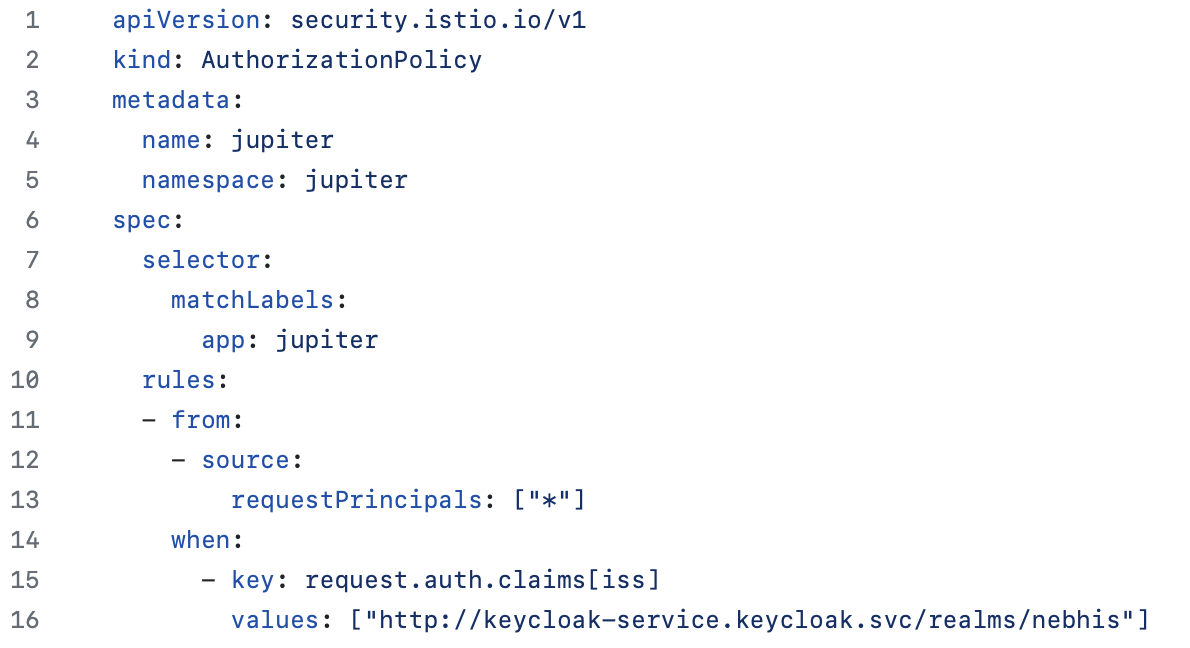
\includegraphics[width=10cm]{./images/authorizationpolicy}
  \caption{Istio AuthorizationPolicy [source: author]}
  \label{fig:authorizationpolicy}
\end{figure}

\begin{figure}[htbp]
  \centering
      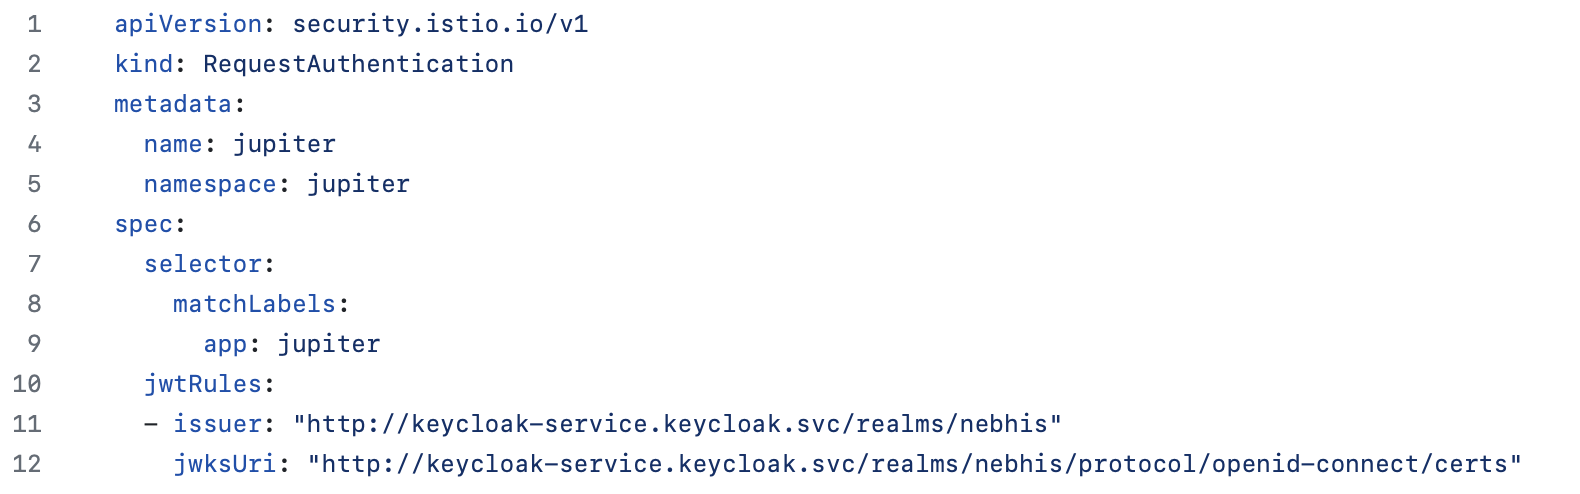
\includegraphics[width=11cm]{./images/requestauthentication}
  \caption{Istio RequestAuthentication [source: author]}
  \label{fig:requestauthentication}
\end{figure}

\newpage
\section{Cluster End Result}

To mimick actual business software hosted... 

examples with Neptune and Jupiter settings, python script, kubectl get pods --all-namespaces, etc

Notice how Neptune and Jupiter as actual application-pods show 2/2. App container and sidecar

\begin{figure}[htbp]
  \centering
      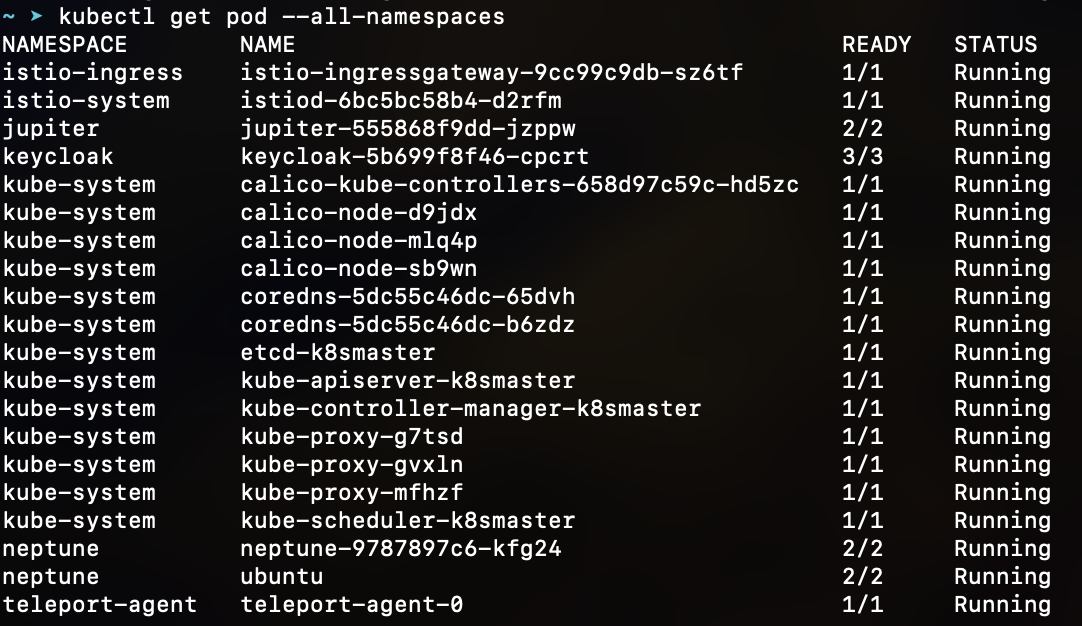
\includegraphics[width=10cm]{./images/finalcluster}
  \caption{All pods of the final cluster [source: author]}
  \label{fig:finalcluster}
\end{figure}

\newpage
Neptune calling Jupiter by first obtaining JWT token from Keycloak

\newpage
\chapter{Discussion and Future Work}

There is still much more that can be done to ensure a fully production grade environment constructed after the idea of Zero Trust. 
This includes certificate management, container image scanning and the establishment of general cluster policies that need to be met before resources can even be 
applied to the cluster. However, this thesis comprehensively covers the core ideas of ZT, for example how the elimination of implicit trust between participating parties 
can be achieved. If an attacker was to gain access to a kubeconfig, it would only be valid for the duration of the Teleport session.
If an attacker was to gain access to a pod, they would be significantly restricted in their actions by network segmentation as well as Istio's 
traffic controlling policies tightly integrated with Keycloak's Identity and Access Management. The only disadavntage of Istio is the added strain on cluster resources, 
since every deployment is accompanied a sidecar process. 
To enhance the security posture of the environment even more, secret management is another critical aspect to consider. Secrets such as database credentials and 
API keys, SSL certificates and SSL keys used by applications deployed in Kubernetes, must be externalized from the source code and repository platforms like GitHub. 
The self-hosted open-source tool Hashicorp Vault can be utilized to store for example the client credentials of applications used to retrieve OIDC tokens from Keycloak.
Only at startup this client credential is loaded into the application container, which ensures that sensitive information is secured at rest. 
Also, there can be even more focus placed on the ZT importance of auditing. Log collectors and aggregators could standardize the output stream of audit logs provided by Teleport, Istio and Keycloak,
summarize and report them. 
\newline
\newline
Another improvement that could be made to the setup is the usage of Infrastructure as Code and GitOps. With Iac, the Kubernetes VMs could be managed and provisioned using machine-readable
configuration files as done in Ansible, rather than manually issuing interactive commands or doing bash scripting. GitOps is a set of practices that uses Git repositories as the single source of truth for 
infrastructure and applications, enabling automated deployments and operational tasks through pull requests and continuous delivery pipelines. Tools like Flux and ArgoCD can 
continuously synchronize the environement's state from a Git repository. This way, the environment is standardized, centralized and always replicable in case it needs to be brought down or migrated
due to system failure or compromise by malicious actors.
\newline
\newline
Furthermore, AI-driven threat detection has made significant progress in recent years. In AI-driven threat detection, machine learning algorithms identify a baseline of normal network behavior.
If the behavior on the network deviates from this usual state, a potential security threat might be alerted. At such a point, these kind of AI-driven systems can automate the incident response 
and block IP addresses, apply policies, deploy patches and notify system administrators on their own accord. As a dataset, network traffic logs from Istio's sidecars could be fed into such machine learning models.
Evidently, there is always room for improvement and there will always be ways to elevate the security standard of a Kubernetes cluster and an infrastructure in general, especially
due to fast changing landsacape IT security and Kubernetes. Thus, future work might build on top of this setup and concern itself with the exact critiques laid out above. 


\newpage
\chapter{Conclusion}

This thesis aims to construct a Kubernetes cluster inspired by Zero Trust principles according to NIST Special Publication 800-207. Before concrete implementation is executed, 
viable technologies are first compared based on factors which are important to fulfill Zero Trust requirements. The significance of this work lies in its practical demonstration of 
applying Zero Trust principles to a Kubernetes environment, providing a blueprint for enhancing security in modern containerized applications. Teleport, Istio and Keycloak are set up as
central components of the cluster, providing MFA, microsegementation, minimal access, continuous verification and more. In a production context, provided with ZT principles and recommendations, 
one must evaluate the granularity of policies and the strictness of the environment as a whole, as well as find the balance between developer restriction and security. There is no definite checklist
to tick off after which one can expect to have a 100\% Zero Trust Kubernetes environment. Applying ZT to Kubernetes is a continuous process assessing the security posture of the environment and making the necessary 
adaptations. 



\newpage

% --- Bibliography ------------------------------------------------------

%IEEE Citation [1]
\bibliographystyle{IEEEtran}
%for alphanumeric citation eg.: [ABC19]
%\bibliographystyle{alpha}

% List references I definitely want in the bibliography,
% regardless of whether or not I cite them in the thesis.

\newpage
\addcontentsline{toc}{chapter}{Bibliography}
\bibliography{testBib}

\newpage

% --- List of Figures ----------------------------------------------------

\addcontentsline{toc}{chapter}{List of Figures}
\listoffigures


% --- List of Tables -----------------------------------------------------

% --- Appendix A -----------------------------------------------------


\end{document}
